\chapter{单纯形法}
\label{chap:simplex-method}

一家工厂用三种有限的资源生产两种产品，要定下各生产多少，使利润最大。第~\ref{chap:linear-programming}章说明，这类线性规划若有最优解，就有一个最优解落在可行域的顶点上，而且顶点可以用线性代数写成基本可行解。顶点的个数有限，却可能极多，逐个比较并不可行。\term{单纯形法}（simplex method）的做法是从一个顶点出发，每次沿一条能改善目标的边走到相邻顶点，直到手里拿到一张能证明“不必再走”的凭证。

本章用同一个工厂例子把这件事算到底。先建立一次换基怎样算、什么时候可以停；再回答第一个顶点从哪里来，遇到几条约束挤在同一个顶点时会发生什么，以及大规模问题上这些计算怎样组织。有了最优基之后，还能在资源或价格变化时复用它：对偶单纯形法从失去可行性的基接着求解，固定基的参数分析则直接读出结论成立的范围。最后一节用一族构造好的例子说明，换基的次数在最坏情形下可以随维数指数增长。

\section{换基与最优性判别}
\label{sec:simplex-basis-exchange}

手里已经有一个可行的顶点时，怎样判断它是不是最优；如果不是，下一步该走到哪里？

\paragraph{一个资源配置问题}
工厂生产两种产品，产量分别记为$x_1,x_2$，单位利润分别是$4$和$5$。原料有$8$单位，工时有$10$单位，产品二还要占用一台专用设备，设备最多加工$3$单位。两种产品对原料和工时的消耗写在下面的约束里，于是问题是
\begin{equation}
 \begin{aligned}
 \max_{x_1,x_2}\quad & 4x_1+5x_2\\
 \text{s.t.}\quad & x_1+2x_2\leq 8,\\
 & 2x_1+x_2\leq 10,\\
 & x_2\leq 3,\qquad x_1,x_2\geq 0.
 \end{aligned}
 \label{eq:simplex-resource-problem}
\end{equation}
图~\ref{fig:simplex-resource-vertices}画出它的可行域，这是一个有五个顶点的多边形。虚线是利润的等值线，沿箭头方向利润增大，最后离开多边形的那个点就是最优解。

\begin{BookInlineFigure}
 \centering
 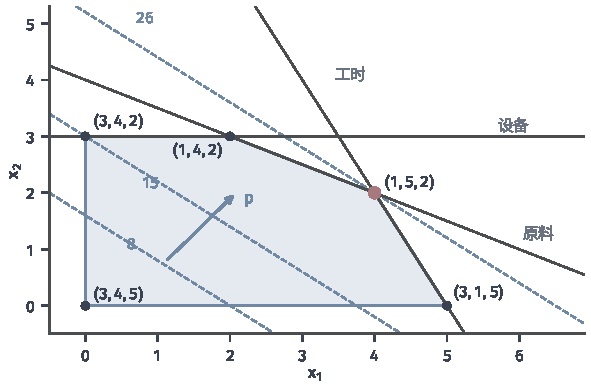
\includegraphics[width=100mm]{figures/05-optimization/01-linear-programming/matplotlib/simplex-resource-vertices/figure.pdf}
 \caption{资源配置问题~\eqref{eq:simplex-resource-problem}的可行域（浅蓝）。三条深灰线分别是原料、工时和设备约束的边界，蓝色虚线是利润$4x_1+5x_2$取$8,15,26$的等值线，箭头$\bm{p}=(4,5)$指向利润增大的方向。每个顶点旁的三元组是它对应的基，红点是最优顶点$(4,2)$。}
 \label{fig:simplex-resource-vertices}
\end{BookInlineFigure}

二维时用眼睛就能找到最优点，但变量一多就画不出来，需要把“在顶点上看哪条边更好”翻译成矩阵运算。先引入松弛变量$x_3,x_4,x_5\geq0$，分别表示没有用完的原料、工时和设备能力，并把最大化改写成最小化，得到第~\ref{chap:linear-programming}章的标准型
\begin{equation}
 \min_{\bm{x}}\ \bm{c}^\top\bm{x}\quad\text{s.t.}\quad \bm{A}\bm{x}=\bm{b},\quad \bm{x}\geq\bm{0},
 \label{eq:simplex-standard-form}
\end{equation}
其中$\bm{A}\in\mathbb{R}^{m\times n}$满行秩，第$j$列记为$\bm{a}_j=\bm{A}_{:,j}$。本例中$m=3$，$n=5$，数据是
\begin{equation}
 \bm{A}=\begin{bmatrix}1&2&1&0&0\\2&1&0&1&0\\0&1&0&0&1\end{bmatrix},\quad
 \bm{b}=\begin{bmatrix}8\\10\\3\end{bmatrix},\quad
 \bm{c}=\begin{bmatrix}-4\\-5\\0\\0\\0\end{bmatrix}.
 \label{eq:simplex-resource-data}
\end{equation}
最小化的目标值$f=\bm{c}^\top\bm{x}$是负的利润，所以下文中$f$越小，利润越大。

\paragraph{基与顶点}
第~\ref{chap:linear-programming}章已经建立了下面要用的事实。取$m$个下标组成有序元组$B$，使基矩阵$\bm{A}_B$可逆，这样的$B$称为基，其余下标组成$N$。令非基分量为零，基分量为
\[
 \bm{x}_B=\bm{A}_B^{-1}\bm{b},\qquad \bm{x}_N=\bm{0},
\]
就得到一个基本解。$\bm{x}_B\geq\bm{0}$时它是基本可行解，也就是可行域的极点；问题可行且最优值有限时，最优解可以在基本可行解中取得。所以只需在基之间搜索。下标属于$B$的变量称为\term{基变量}（basic variable），其余的称为\term{非基变量}（nonbasic variable）。

以顶点$(4,2)$为例，此时原料和工时恰好用完，即$x_3=x_4=0$，而设备还余$x_5=1$。非基变量是$x_3,x_4$，基变量是$x_1,x_5,x_2$，我们把基写成$B=(1,5,2)$。元组的顺序用来对应$\bm{x}_B$的分量，换基时新变量占据被换出变量的位置，顺序因此保持稳定。

\paragraph{主要思想：用非基变量表示一切}
站在一个顶点上，我们想知道沿每条边走会怎样。非基变量恰好提供了一组局部坐标：它们此刻都是零，让其中一个变大，就是离开顶点走上一条边。因此要把基变量和目标都写成非基变量的函数。

把$\bm{A}\bm{x}=\bm{b}$按基和非基拆开，得到$\bm{A}_B\bm{x}_B+\bm{A}_N\bm{x}_N=\bm{b}$。两边左乘$\bm{A}_B^{-1}$，每个满足等式约束的点都有
\begin{equation}
 \bm{x}_B=\bm{A}_B^{-1}\bm{b}-\bm{A}_B^{-1}\bm{A}_N\bm{x}_N.
 \label{eq:simplex-basic-form}
\end{equation}
代入目标后，整理非基变量的系数：
\[
 \bm{c}^\top\bm{x}
 =\bm{c}_B^\top\bm{x}_B+\bm{c}_N^\top\bm{x}_N
 =\bm{c}_B^\top\bm{A}_B^{-1}\bm{b}
 +\bigl(\bm{c}_N^\top-\bm{c}_B^\top\bm{A}_B^{-1}\bm{A}_N\bigr)\bm{x}_N.
\]

系数里反复出现$\bm{c}_B^\top\bm{A}_B^{-1}$，把它单独命名。记
\begin{equation}
 \bm{y}=\bm{A}_B^{-\top}\bm{c}_B,
 \qquad
 s_j=c_j-\bm{a}_j^\top\bm{y}\quad(j=1,\ldots,n),
 \label{eq:simplex-reduced-cost}
\end{equation}
其中$\bm{y}\in\mathbb{R}^m$称为这个基的对偶候选，$s_j$称为$x_j$的\term{约化成本}（reduced cost）。对基变量，$\bm{A}_B^\top\bm{y}=\bm{c}_B$正好说明$s_j=0$（$j\in B$）。于是每个满足等式约束的点都有
\begin{equation}
 \bm{c}^\top\bm{x}=\bm{b}^\top\bm{y}+\sum_{j\in N}s_jx_j.
 \label{eq:simplex-objective-form}
\end{equation}

这个式子是本章的出发点。第一项是当前顶点的目标值，第二项说明：让非基变量$x_j$从零增加一个单位，目标改变$s_j$。可以这样理解这些量：$y_i$是这个基给第$i$种资源定的内部单价，$\bm{a}_j^\top\bm{y}$是生产一单位$x_j$所耗资源按内部单价折算的总价，$s_j$是$x_j$的真实成本减去这个折算价。$s_j<0$表示真实成本比折算价低，做这件事划算。

这组记号和第~\ref{chap:linear-programming}章的对偶是同一套。对偶问题要求$\bm{A}^\top\bm{y}+\bm{s}=\bm{c}$且$\bm{s}\geq\bm{0}$，而式~\eqref{eq:simplex-reduced-cost}总满足前一半，只差$\bm{s}\geq\bm{0}$。“候选”二字指的就是这一点：等式已经成立，符号条件还要检查。

\begin{theorem}[最优性判别]
 \label{thm:simplex-optimality}
 设$B$是可行基，基本可行解为$\bar{\bm{x}}$，$\bm{y},\bm{s}$由式~\eqref{eq:simplex-reduced-cost}给出。若
 \begin{equation}
  s_j\geq 0\quad\text{对所有 }j\in N\text{ 成立},
  \label{eq:simplex-optimality-condition}
 \end{equation}
 则$\bar{\bm{x}}$是标准型~\eqref{eq:simplex-standard-form}的全局最优解，$(\bm{y},\bm{s})$是对偶最优解，两者目标值相等。
\end{theorem}

\begin{proof}
 任取可行点$\bm{x}$。它满足$\bm{A}\bm{x}=\bm{b}$，所以式~\eqref{eq:simplex-objective-form}对它成立。又因$\bm{x}_N\geq\bm{0}$且$s_j\geq0$，右端第二项非负，于是
 \[
  \bm{c}^\top\bm{x}\geq\bm{b}^\top\bm{y}.
 \]
 另一方面$\bar{\bm{x}}_N=\bm{0}$，式~\eqref{eq:simplex-objective-form}给出$\bm{c}^\top\bar{\bm{x}}=\bm{b}^\top\bm{y}$。所以$\bar{\bm{x}}$的目标值不大于任何可行点的目标值。条件~\eqref{eq:simplex-optimality-condition}连同基变量的$s_j=0$说明$(\bm{y},\bm{s})$对偶可行，它的对偶目标$\bm{b}^\top\bm{y}$等于原始目标，由弱对偶知它是对偶最优解。
\end{proof}

判别只看当前顶点的约化成本，结论却是全局的，原因在于式~\eqref{eq:simplex-objective-form}对所有满足等式的点都成立，不是局部近似。约化成本全部非负，就等于对偶可行，$\bm{y}$就是第~\ref{chap:linear-programming}章说的下界证书。

定理的方向只有一个：非负是最优的充分条件。某个$s_j<0$时，当前顶点是否一定不是最优，要看沿这条边能否真的走出去，这正是下面要讨论的。

\paragraph{主要思想：沿一条边走到下一个顶点}
设$s_q<0$，$q\in N$，我们让$x_q$增大，其余非基变量保持为零。记增大的幅度为$\alpha\geq0$，由式~\eqref{eq:simplex-basic-form}，基变量随之按下式变化：
\begin{equation}
 \bm{x}_B(\alpha)=\bar{\bm{x}}_B-\alpha\bm{u},\qquad \bm{u}=\bm{A}_B^{-1}\bm{a}_q.
 \label{eq:simplex-direction}
\end{equation}
$\bm{u}$的含义很具体：$u_i$是$x_q$每增加一单位时，位于第$i$个位置的基变量要减少的量。用整个向量来写，移动方向$\bm{d}\in\mathbb{R}^n$满足$d_q=1$，$\bm{d}_B=-\bm{u}$，其余分量为零。

沿这个方向走，等式约束不被破坏，目标按$s_q$下降。两件事都可以直接验算：
\[
 \bm{A}\bm{d}=\bm{a}_q-\bm{A}_B\bm{u}=\bm{0},
 \qquad
 \bm{c}^\top\bm{d}=c_q-\bm{c}_B^\top\bm{A}_B^{-1}\bm{a}_q=s_q.
\]

图~\ref{fig:simplex-edge-rates}在顶点$(2,3)$上画出了这两种可能。这个顶点的基是$(1,4,2)$，$x_3,x_5$非基。让$x_3$增大，点沿设备约束的边向左移动，目标以速率$s_3=4$变差；让$x_5$增大，点沿原料约束的边向右下移动，目标以速率$s_5=-3$变好。

\begin{BookInlineFigure}
 \centering
 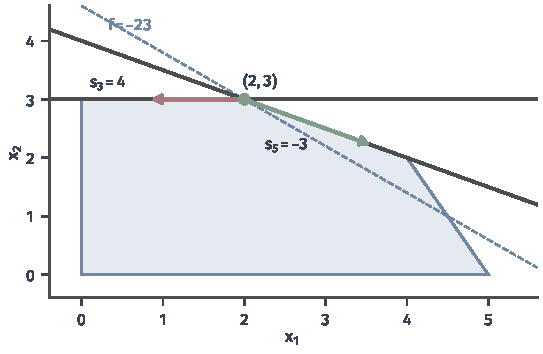
\includegraphics[width=92mm]{figures/05-optimization/01-linear-programming/matplotlib/simplex-edge-rates/figure.pdf}
 \caption{顶点$(2,3)$处的两条边。深灰粗线是在此活动的设备和原料约束，蓝色虚线是过该点的等值线$f=-23$。红色箭头是$x_3$增大的方向，走上去$f$每单位增加$4$；绿色箭头是$x_5$增大的方向，走上去$f$每单位减少$3$，它越过等值线进入利润更高的一侧。}
 \label{fig:simplex-edge-rates}
\end{BookInlineFigure}

能走多远由基变量的非负性决定。$u_i\leq0$的基变量不会减小，不构成限制；$u_i>0$的基变量在$\alpha=\bar{x}_{B(i)}/u_i$时降到零，其中$B(i)$是基中第$i$个下标。最先降到零的那个变量决定步长：
\begin{equation}
 \alpha^\star=\min_{i:\,u_i>0}\frac{\bar{x}_{B(i)}}{u_i}.
 \label{eq:simplex-ratio-test}
\end{equation}
这称为\term{比值检验}（ratio test）。像预算线一样，每种资源各自算出“还够做多少”，能做的量由最紧的那一种决定。图~\ref{fig:simplex-ratio-test}把基变量画成$\alpha$的直线，第一条碰到零的直线给出步长。

\begin{BookInlineFigure}
 \centering
 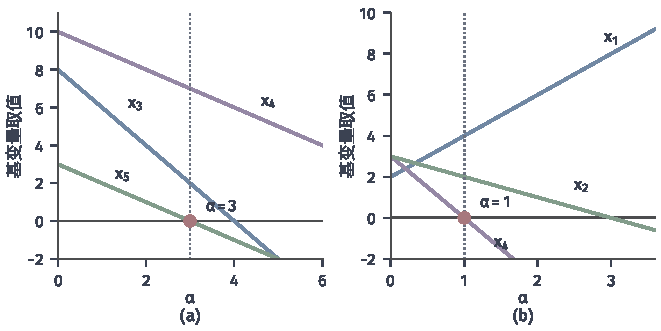
\includegraphics[width=112mm]{figures/05-optimization/01-linear-programming/matplotlib/simplex-ratio-test/figure.pdf}
 \caption{比值检验的两个实例，三条直线是基变量随步长$\alpha$的变化，红点是最先降到零的位置。(a)~入基变量$x_2$，基$(3,4,5)$，$x_5$先到零，$\alpha^\star=3$。(b)~入基变量$x_5$，基$(1,4,2)$，$x_1$随$\alpha$增大而增大，不起限制作用，$x_4$先到零，$\alpha^\star=1$。}
 \label{fig:simplex-ratio-test}
\end{BookInlineFigure}

设最小值在位置$r$取到，$p=B(r)$。走到$\alpha^\star$后$x_p=0$，$x_q=\alpha^\star$，于是把$p$从基中换出、$q$换入。$x_q$称为\term{入基变量}（entering variable），$x_p$称为\term{出基变量}（leaving variable），这一次替换称为\term{换基}（pivot）。下面的引理保证替换后仍是一个可行基。

\begin{lemma}[换基的合法性]
 \label{lem:simplex-pivot}
 设$s_q<0$，$\bm{u}$由式~\eqref{eq:simplex-direction}给出且$\bm{u}$至少有一个正分量，$r$在式~\eqref{eq:simplex-ratio-test}中取到最小值。把$B$的第$r$个下标换成$q$，得到的$B'$仍是基，$\bar{\bm{x}}+\alpha^\star\bm{d}$是它的基本可行解，目标值为
 \begin{equation}
  \bm{c}^\top\bar{\bm{x}}+\alpha^\star s_q.
  \label{eq:simplex-objective-update}
 \end{equation}
\end{lemma}

\begin{proof}
 先证$\bm{A}_{B'}$可逆。由$\bm{A}_B\bm{u}=\bm{a}_q$，有$\bm{a}_q=\sum_iu_i\bm{a}_{B(i)}$，其中$\bm{a}_{B(r)}$的系数$u_r>0$。若$\bm{A}_{B'}$的列线性相关，由于其余$m-1$列线性无关，$\bm{a}_q$就能只用这$m-1$列表示，这与$\bm{a}_q$在基$\bm{A}_B$下表示的唯一性及$u_r\neq0$矛盾。

 再看新点。由$\bm{A}\bm{d}=\bm{0}$，等式约束保持成立。$\alpha^\star$的取法使所有基变量非负，$x_q=\alpha^\star\geq0$。新点在位置$p$和$N\setminus\{q\}$上的分量都是零，也就是$B'$之外的分量都是零，所以它是$B'$的基本可行解。目标值由$\bm{c}^\top\bm{d}=s_q$得到。
\end{proof}

$\alpha^\star>0$时，目标严格下降，点从一个顶点沿边走到了相邻顶点。这就是单纯形法的全部几何内容。

\needspace{6\baselineskip}
\paragraph{变量}
下面用工厂的例子走完整个过程。计算中出现的量及其形状如下。
\begin{itemize}
 \item $B^{(t)}$：第$t$轮的基，含$m$个下标的有序元组；$N^{(t)}$是其余$n-m$个下标。
 \item $\bm{x}_B^{(t)}\in\mathbb{R}^m$：基变量的取值，非基变量都是零。
 \item $\bm{y}^{(t)}\in\mathbb{R}^m$：对偶候选。
 \item $s_j^{(t)}$：非基变量的约化成本。
 \item $q^{(t)}$：入基下标；$\bm{u}^{(t)}\in\mathbb{R}^m$：入基列在当前基下的表示。
 \item $\alpha^{(t)}\geq0$：步长；$r^{(t)}$：出基位置，$p^{(t)}=B^{(t)}(r^{(t)})$是出基下标。
\end{itemize}

\paragraph{初始化}
需要一个可行基$B^{(0)}$。当$\bm{b}\geq\bm{0}$且每个约束都带松弛变量时，取全部松弛变量为基即可，此时$\bm{A}_B=\bm{I}$。其他情形在第~\ref{sec:simplex-initial-basis}节处理。例中
\[
 B^{(0)}=(3,4,5),\qquad \bm{A}_{B^{(0)}}=\bm{I},\qquad \bm{x}_B^{(0)}=\begin{bmatrix}8\\10\\3\end{bmatrix}.
\]
对应顶点$(0,0)$，什么都不生产，$f=0$。

\needspace{6\baselineskip}
\paragraph{每轮更新}
第$t$轮依次做下面几步。步骤后的“例中”是第$0$轮的数据，其余各轮随后列出。
\begin{enumerate}

 \item 计算对偶候选。由式~\eqref{eq:simplex-reduced-cost}，
 \[
  \bm{y}^{(t)}=\bigl(\bm{A}_{B^{(t)}}\bigr)^{-\top}\bm{c}_{B^{(t)}}.
 \]
 例中$\bm{c}_B=\bm{0}$，所以
 \[
  \bm{y}^{(0)}=(0,0,0)^\top.
 \]

 \item 定价，即对每个非基下标计算约化成本$s_j^{(t)}=c_j-\bm{a}_j^\top\bm{y}^{(t)}$。例中
 \[
  s_1^{(0)}=-4,\qquad s_2^{(0)}=-5.
 \]

 \item 判别。若所有$s_j^{(t)}\geq0$，停止，当前解最优。否则选一个$s_q^{(t)}<0$的下标$q=q^{(t)}$入基。本节取约化成本最负的下标，称为\term{Dantzig规则}（Dantzig's rule），并列时取下标最小者。例中$s_2$最负，所以
 \[
  q^{(0)}=2.
 \]

 \item 计算入基列的表示。由式~\eqref{eq:simplex-direction}，
 \[
  \bm{u}^{(t)}=\bigl(\bm{A}_{B^{(t)}}\bigr)^{-1}\bm{a}_q.
 \]
 若$\bm{u}^{(t)}\leq\bm{0}$，停止，问题无界。例中
 \[
  \bm{u}^{(0)}=\bm{a}_2=(2,1,1)^\top.
 \]

 \item 比值检验。由式~\eqref{eq:simplex-ratio-test}求$\alpha^{(t)}$和出基位置$r^{(t)}$，并列时本节取下标最小的基变量。例中三个比值是
 \[
  \frac{x_3}{u_1}=\frac{8}{2}=4,\qquad
  \frac{x_4}{u_2}=\frac{10}{1}=10,\qquad
  \frac{x_5}{u_3}=\frac{3}{1}=3,
 \]
 所以
 \[
  \alpha^{(0)}=3,\qquad r^{(0)}=3,\qquad p^{(0)}=5.
 \]

 \item 更新基和基变量。除第$r$个位置外，
 \begin{equation}
  \bm{x}_B^{(t+1)}=\bm{x}_B^{(t)}-\alpha^{(t)}\bm{u}^{(t)},
  \label{eq:simplex-primal-update}
 \end{equation}
 第$r$个位置改放$x_q=\alpha^{(t)}$，并把$B^{(t)}$的第$r$个下标换成$q$。例中
 \[
  B^{(1)}=(3,4,2),\qquad \bm{x}_B^{(1)}=\begin{bmatrix}8-3\cdot2\\10-3\cdot1\\3\end{bmatrix}=\begin{bmatrix}2\\7\\3\end{bmatrix}.
 \]
 目标值由式~\eqref{eq:simplex-objective-update}变为$0+3\cdot(-5)=-15$，点走到$(0,3)$。
\end{enumerate}

例中第$1$轮的基矩阵是
\[
 \bm{A}_{B^{(1)}}=\begin{bmatrix}1&0&2\\0&1&1\\0&0&1\end{bmatrix}.
\]
解$\bm{A}_B^\top\bm{y}=\bm{c}_B$，其中$\bm{c}_B=(0,0,-5)^\top$，再计算两个非基变量的约化成本：
\[
 \bm{y}^{(1)}=(0,0,-5)^\top,\qquad s_1^{(1)}=-4,\qquad s_5^{(1)}=5.
\]
只有$s_1<0$，所以$x_1$入基。它的表示和两个有效比值为
\[
 \bm{u}^{(1)}=(1,2,0)^\top,\qquad
 \frac{x_3}{u_1}=\frac{2}{1}=2,\qquad
 \frac{x_4}{u_2}=\frac{7}{2}.
\]
第三个分量$u_3=0$，产品一不占专用设备，$x_2$不受影响。于是$\alpha^{(1)}=2$，$x_3$出基，更新后
\[
 B^{(2)}=(1,4,2),\qquad \bm{x}_B^{(2)}=\begin{bmatrix}2\\7-2\cdot2\\3\end{bmatrix}=\begin{bmatrix}2\\3\\3\end{bmatrix}.
\]
目标值变为$-15+2\cdot(-4)=-23$，点走到$(2,3)$。

例中第$2$轮的基矩阵和对偶候选是
\[
 \bm{A}_{B^{(2)}}=\begin{bmatrix}1&0&2\\2&1&1\\0&0&1\end{bmatrix},\qquad
 \bm{c}_B=\begin{bmatrix}-4\\0\\-5\end{bmatrix},\qquad
 \bm{y}^{(2)}=\begin{bmatrix}-4\\0\\3\end{bmatrix}.
\]
非基变量$x_3,x_5$的约化成本为
\[
 s_3^{(2)}=0-(-4)=4,\qquad s_5^{(2)}=0-3=-3.
\]
这里出现了一个值得留意的现象：$x_5$是设备的余量，让它入基意味着故意不用满设备。$s_5<0$说明把设备让出一些，腾出的原料拿去做产品一更赚钱。$x_5$入基，表示向量和比值为
\[
 \bm{u}^{(2)}=(-2,3,1)^\top,\qquad
 \frac{x_4}{u_2}=\frac{3}{3}=1,\qquad
 \frac{x_2}{u_3}=\frac{3}{1}=3.
\]
$u_1=-2<0$表示$x_1$会增大，不参与比较。于是$\alpha^{(2)}=1$，$x_4$出基，按式~\eqref{eq:simplex-primal-update}更新：
\[
 B^{(3)}=(1,5,2),\qquad
 \bm{x}_B^{(3)}=\begin{bmatrix}2+2\\1\\3-1\end{bmatrix}=\begin{bmatrix}4\\1\\2\end{bmatrix}.
\]
目标值变为$-23+1\cdot(-3)=-26$，点走到$(4,2)$。

例中第$3$轮的基矩阵和对偶候选是
\[
 \bm{A}_{B^{(3)}}=\begin{bmatrix}1&0&2\\2&0&1\\0&1&1\end{bmatrix},\qquad
 \bm{c}_B=\begin{bmatrix}-4\\0\\-5\end{bmatrix},\qquad
 \bm{y}^{(3)}=\begin{bmatrix}-2\\-1\\0\end{bmatrix}.
\]
非基变量$x_3,x_4$的约化成本为
\[
 s_3^{(3)}=0-(-2)=2,\qquad s_4^{(3)}=0-(-1)=1.
\]
两者都非负，算法停止。表~\ref{tab:simplex-resource-rounds}汇总了四轮的数据。

\begin{BookInlineTable}
 \centering
 \begin{tabular}{cccccc}
  \toprule
  $t$ & $B^{(t)}$ & $(x_1,x_2)$ & $f$ & $\bm{y}^{(t)}$ & 入基／出基\\
  \midrule
  $0$ & $(3,4,5)$ & $(0,0)$ & $0$ & $(0,0,0)$ & $x_2$／$x_5$\\
  $1$ & $(3,4,2)$ & $(0,3)$ & $-15$ & $(0,0,-5)$ & $x_1$／$x_3$\\
  $2$ & $(1,4,2)$ & $(2,3)$ & $-23$ & $(-4,0,3)$ & $x_5$／$x_4$\\
  $3$ & $(1,5,2)$ & $(4,2)$ & $-26$ & $(-2,-1,0)$ & 停止\\
  \bottomrule
 \end{tabular}
 \caption{资源配置问题在Dantzig规则下的各轮数据。}
 \label{tab:simplex-resource-rounds}
\end{BookInlineTable}

\paragraph{最终得到}
算法结束时得到最优基$B^\star=(1,5,2)$和最优解
\begin{equation}
 \bm{x}^\star=(4,2,0,0,1)^\top,\qquad p^\star=-26,
 \label{eq:simplex-resource-solution}
\end{equation}
即产品一做$4$、产品二做$2$，利润$26$，原料和工时用完，设备余$1$。同时得到对偶最优解
\begin{equation}
 \bm{y}^\star=(-2,-1,0)^\top,\qquad \bm{s}^\star=(0,0,2,1,0)^\top.
 \label{eq:simplex-resource-dual}
\end{equation}
证书可以当场核对：一方面$\bm{b}^\top\bm{y}^\star=-16-10=-26=p^\star$，另一方面$(\bm{x}^\star)^\top\bm{s}^\star=0$，互补松弛成立。

几何上，最优性说的是目标方向落在活动约束法向量张成的锥里。把最大化写回去，利润向量恰好是原料和工时两个法向量的非负组合：
\[
 \begin{bmatrix}4\\5\end{bmatrix}=2\begin{bmatrix}1\\2\end{bmatrix}+1\begin{bmatrix}2\\1\end{bmatrix}.
\]
图~\ref{fig:simplex-optimal-cone}画的就是这个分解，组合系数$2,1$正是$-\bm{y}^\star$的前两个分量。

\begin{BookInlineFigure}
 \centering
 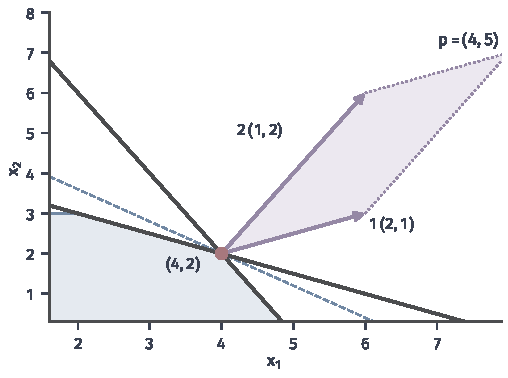
\includegraphics[width=86mm]{figures/05-optimization/01-linear-programming/matplotlib/simplex-optimal-cone/figure.pdf}
 \caption{最优顶点$(4,2)$处的对偶证书。深灰粗线是两条活动约束，紫色箭头是它们的法向量按系数$2$和$1$缩放后的结果，蓝色箭头是利润向量$\bm{p}$，它是紫色平行四边形的对角线，因此落在两个法向量张成的锥内。蓝色虚线是过该点的等值线。}
 \label{fig:simplex-optimal-cone}
\end{BookInlineFigure}

\paragraph{换基规则影响路径，不影响结论}
Dantzig规则只看单位变化率，不看能走多远。图~\ref{fig:simplex-vertex-paths}对比了同一问题上的两条路径：Dantzig规则先选利润系数大的$x_2$，走了三步；若总选下标最小的负约化成本，则先选$x_1$，经$(5,0)$两步到达。两条路径终点相同，因为最优性判别不依赖路径。这个例子不能说明后一种规则更好，它只说明步数取决于规则与问题的搭配。

\begin{BookInlineFigure}
 \centering
 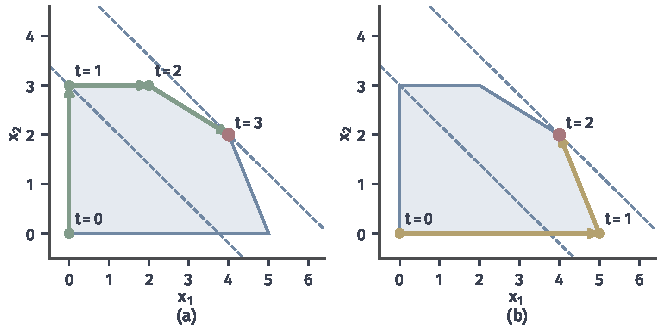
\includegraphics[width=112mm]{figures/05-optimization/01-linear-programming/matplotlib/simplex-vertex-paths/figure.pdf}
 \caption{同一问题上的两条换基路径，蓝色虚线是利润$15$和$26$的等值线，红点是最优解。(a)~Dantzig规则（绿色），经$(0,3)$和$(2,3)$共三次换基。(b)~总选下标最小的负约化成本（黄色），经$(5,0)$共两次换基。}
 \label{fig:simplex-vertex-paths}
\end{BookInlineFigure}

\paragraph{没有出基变量：无界证书}
比值检验可能找不到任何限制。此时$\bm{u}\leq\bm{0}$，对一切$\alpha\geq0$，$\bar{\bm{x}}+\alpha\bm{d}$都可行，目标按$\alpha s_q$趋于$-\infty$。这个$\bar{\bm{x}}$和$\bm{d}$合在一起就是问题无下界的证据：
\begin{equation}
 \bm{A}\bm{d}=\bm{0},\qquad \bm{d}\geq\bm{0},\qquad \bm{c}^\top\bm{d}=s_q<0.
 \label{eq:simplex-unbounded-certificate}
\end{equation}

\begin{example}[无界问题]
 \label{ex:simplex-unbounded}
 考虑最大化$x_1+x_2$，约束为$x_1-x_2\leq2$，$-x_1+x_2\leq1$，$x_1,x_2\geq0$。加松弛变量$x_3,x_4$，从$B=(3,4)$出发，约化成本是$s_1=s_2=-1$，取$x_1$入基。比值检验给出$x_3$出基，$\alpha=2$，点到达$(2,0)$。

 第二轮$B=(1,4)$，对偶候选和约化成本为
 \[
  \bm{y}=(-1,0)^\top,\qquad s_2=-2,\qquad s_3=1.
 \]
 $x_2$入基，它的表示是
 \[
  \bm{u}=(-1,0)^\top\leq\bm{0}.
 \]
 没有基变量会减小，比值检验无从进行。按式~\eqref{eq:simplex-unbounded-certificate}得到无界方向$\bm{d}=(1,1,0,0)^\top$，沿它每走一单位，目标减少$2$。
\end{example}

图~\ref{fig:simplex-unbounded}中可行域是一条向右上方延伸的带子，红色射线在带子里一直走不出去，而利润不断增大。

\begin{BookInlineFigure}
 \centering
 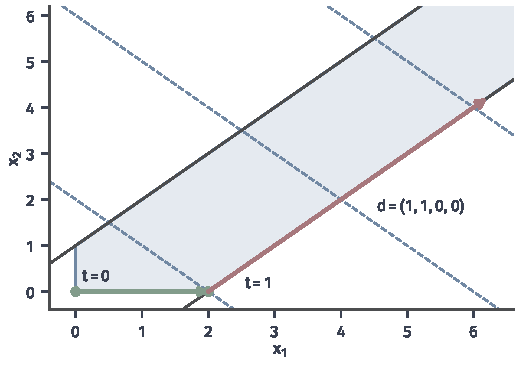
\includegraphics[width=88mm]{figures/05-optimization/01-linear-programming/matplotlib/simplex-unbounded/figure.pdf}
 \caption{例~\ref{ex:simplex-unbounded}的无界可行域（浅蓝，向右上方无限延伸）。绿色是一次换基，从$(0,0)$到$(2,0)$；红色射线是无界方向$\bm{d}$，蓝色虚线是利润$2,6,10$的等值线，射线不断穿过利润更高的等值线。}
 \label{fig:simplex-unbounded}
\end{BookInlineFigure}

\paragraph{走不动的换基}
还有一种情形需要先记下来。若某个基变量已经是零，且它对应的$u_i>0$，式~\eqref{eq:simplex-ratio-test}给出$\alpha^\star=0$。这时基换了，点没动，目标也没变，这样的基是退化基。所以$s_q<0$只说明这条边的方向改善目标，并不保证真能走出去，$\alpha^\star=0$时当前点可能已经最优。第~\ref{sec:simplex-degeneracy}节专门处理这种情形。

没有退化时，算法的终止性可以直接得出。

\begin{theorem}[非退化时的有限终止]
 \label{thm:simplex-finite-nondegenerate}
 设算法访问的每个基都非退化，则从任一可行基出发，单纯形法经过有限次换基后，或得到满足式~\eqref{eq:simplex-optimality-condition}的最优基，或得到满足式~\eqref{eq:simplex-unbounded-certificate}的无界方向。
\end{theorem}

\begin{proof}
 非退化时$\bar{\bm{x}}_B>\bm{0}$，比值检验给出$\alpha^\star>0$，由式~\eqref{eq:simplex-objective-update}，目标严格下降，所以任何基都不会重复访问。基的个数不超过从$n$个下标中选$m$个的组合数，是有限的，因此换基只能进行有限次。算法每轮要么换基，要么在两种停止条件之一下结束，由此得到结论。
\end{proof}

\section{初始可行基}
\label{sec:simplex-initial-basis}

上一节的算法要从一个可行基出发，而工厂例子里松弛变量恰好提供了一个。本节解决没有现成可行基时怎么办。

给工厂加一个合同要求：两种产品合计至少交付$2$单位，即$x_1+x_2\geq2$。这个不等式要减去一个非负的剩余变量$x_6$才能化成等式，标准型的第四行是
\begin{equation}
 x_1+x_2-x_6=2.
 \label{eq:simplex-order-row}
\end{equation}
若仍取松弛变量和剩余变量组成基，第四行给出$x_6=-2<0$，不可行。这对应图~\ref{fig:simplex-two-phase-path}中的原点：什么都不生产，合同就违约了，原点已不在可行域内。等式约束的情形更直接，它没有松弛变量可用。

\paragraph{人工变量}
解决办法是暂时允许约束被违反，并给违反量记账。把各行乘以适当的符号使$\bm{b}\geq\bm{0}$，对缺少现成基列的行，引入非负的\term{人工变量}（artificial variable）$\bm{v}$，得到扩大的约束
\begin{equation}
 \bm{A}\bm{x}+\bm{v}=\bm{b},\qquad \bm{x}\geq\bm{0},\quad \bm{v}\geq\bm{0}.
 \label{eq:simplex-artificial-system}
\end{equation}
为叙述简单，这里写成每行都加人工变量；已有松弛变量可作基列的行不必加，例中只有第四行需要。

这个系统立刻有可行基：$\bm{x}=\bm{0}$，$\bm{v}=\bm{b}$。但要分清，它是扩大问题的可行基，不是原问题的：只要某个$v_i>0$，对应的原约束就没有被满足。$\bm{v}$像一笔临时垫付的账，只有全部还清，得到的点才是原问题的可行点。

例中把人工变量记作$x_7$，扩大后的约束有四行七列：
\[
 \begin{bmatrix}
 1&2&1&0&0&0&0\\
 2&1&0&1&0&0&0\\
 0&1&0&0&1&0&0\\
 1&1&0&0&0&-1&1
 \end{bmatrix}\bm{x}
 =\begin{bmatrix}8\\10\\3\\2\end{bmatrix}.
\]
起始基$(3,4,5,7)$的基矩阵是单位矩阵，$x_7=2$就是合同的缺口。两阶段法和大M法用两种方式把这笔账还清。

\subsection{两阶段法}
\label{sec:simplex-two-phase}

\paragraph{主要思想}
\term{两阶段法}（two-phase method）把“还清账”和“优化目标”分开。第一阶段暂时不管原目标，只最小化人工变量之和：
\begin{equation}
 \min_{\bm{x},\bm{v}}\ \phi=\bm{1}^\top\bm{v}
 \quad\text{s.t.}\quad
 \bm{A}\bm{x}+\bm{v}=\bm{b},\quad\bm{x}\geq\bm{0},\quad\bm{v}\geq\bm{0}.
 \label{eq:simplex-phase-one}
\end{equation}
这个问题有现成的可行基，目标又以$0$为下界，所以单纯形法不会遇到无界，一定有最优值$\phi^\star\geq0$。它回答了可行性问题。

\begin{theorem}[第一阶段的结论]
 \label{thm:simplex-phase-one}
 原问题$\bm{A}\bm{x}=\bm{b}$，$\bm{x}\geq\bm{0}$可行，当且仅当问题~\eqref{eq:simplex-phase-one}的最优值$\phi^\star=0$。若$\phi^\star>0$，设$\bm{y}$是第一阶段最优基的对偶候选，则
 \begin{equation}
  \bm{A}^\top\bm{y}\leq\bm{0},\qquad \bm{b}^\top\bm{y}=\phi^\star>0,
  \label{eq:simplex-farkas-certificate}
 \end{equation}
 这个$\bm{y}$就是原问题不可行的证书。
\end{theorem}

\begin{proof}
 若原问题有可行点$\bm{x}$，则$(\bm{x},\bm{0})$对问题~\eqref{eq:simplex-phase-one}可行，目标为零，又因$\phi\geq0$，所以$\phi^\star=0$。反过来，$\phi^\star=0$时最优解满足$\bm{v}=\bm{0}$，它的$\bm{x}$部分满足$\bm{A}\bm{x}=\bm{b}$，$\bm{x}\geq\bm{0}$。

 设$\phi^\star>0$。第一阶段的目标系数在$\bm{x}$上是零，于是最优性条件$s_j=0-\bm{a}_j^\top\bm{y}\geq0$说明$\bm{A}^\top\bm{y}\leq\bm{0}$。由定理~\ref{thm:simplex-optimality}，两边目标值相等，即$\bm{b}^\top\bm{y}=\phi^\star$。若存在$\bm{x}\geq\bm{0}$满足$\bm{A}\bm{x}=\bm{b}$，就有
 \[
  0<\bm{b}^\top\bm{y}=\bm{x}^\top\bm{A}^\top\bm{y}\leq0,
 \]
 矛盾，这说明$\bm{y}$确实证明了不可行。
\end{proof}

\paragraph{变量}
第一阶段沿用第~\ref{sec:simplex-basis-exchange}节的全部变量，只是下标范围包括人工变量，目标向量换成在$\bm{x}$上为零、在$\bm{v}$上为一的$\bm{g}$。第二阶段回到原来的$\bm{c}$，并去掉人工变量对应的列。

\paragraph{初始化}
第一阶段从人工变量和可用的松弛变量组成的基出发。例中
\[
 B^{(0)}=(3,4,5,7),\qquad \bm{x}_B^{(0)}=(8,10,3,2)^\top,\qquad \phi=2.
\]

\needspace{6\baselineskip}
\paragraph{每轮更新}
两个阶段的每轮计算都与第~\ref{sec:simplex-basis-exchange}节相同，区别只在目标向量和两阶段之间的衔接。
\begin{enumerate}
 \item 第一阶段按$\bm{g}$运行单纯形法，直到约化成本全部非负。例中第$0$轮的对偶候选和约化成本为
 \[
  \bm{y}^{(0)}=(0,0,0,1)^\top,\qquad s_1=-1,\quad s_2=-1,\quad s_6=1.
 \]
 $s_1,s_2$并列最负，取下标小的$x_1$入基。它的表示和比值为
 \[
  \bm{u}^{(0)}=(1,2,0,1)^\top,\qquad
  \frac{8}{1}=8,\quad \frac{10}{2}=5,\quad \frac{2}{1}=2.
 \]
 于是$\alpha^{(0)}=2$，$x_7$出基，更新后
 \[
  B^{(1)}=(3,4,5,1),\qquad \bm{x}_B^{(1)}=(6,6,3,2)^\top,\qquad\phi=0.
 \]
 第$1$轮人工变量已经出基，$\bm{y}^{(1)}=\bm{0}$，所有$s_j\geq0$，第一阶段结束，得到$\phi^\star=0$和原问题的顶点$(2,0)$。
 \item 判断$\phi^\star$。若$\phi^\star>0$，按定理~\ref{thm:simplex-phase-one}报告不可行并给出$\bm{y}$。例中$\phi^\star=0$，继续。
 \item 处理仍在基中的人工变量（做法见下文）。例中人工变量已经出基，无需处理。
 \item 第二阶段用基$B^{(1)}$和原目标$\bm{c}$继续运行单纯形法。例中三轮的数据如下。
\end{enumerate}

第二阶段第$0$轮，基是$(3,4,5,1)$，$f=-8$。对偶候选和约化成本是
\[
 \bm{y}=(0,0,0,-4)^\top,\qquad s_2=-1,\qquad s_6=-4.
\]
$s_6$最负，$x_6$入基，意味着多交付一些。表示向量和有效比值是
\[
 \bm{u}=(1,2,0,-1)^\top,\qquad \frac{6}{1}=6,\qquad \frac{6}{2}=3.
\]
于是$\alpha=3$，$x_4$出基，更新后
\[
 B=(3,6,5,1),\qquad \bm{x}_B=(3,3,3,5)^\top,\qquad f=-20.
\]

第二阶段第$1$轮，点在$(5,0)$。对偶候选和约化成本是
\[
 \bm{y}=(0,-2,0,0)^\top,\qquad s_2=-3,\qquad s_4=2.
\]
$x_2$入基。表示向量和三个有效比值是
\[
 \bm{u}=\Bigl(\frac32,-\frac12,1,\frac12\Bigr)^\top,\qquad
 \frac{3}{3/2}=2,\quad \frac{3}{1}=3,\quad \frac{5}{1/2}=10.
\]
于是$\alpha=2$，$x_3$出基，更新后
\[
 B=(2,6,5,1),\qquad \bm{x}_B=(2,4,1,4)^\top,\qquad f=-26.
\]

第二阶段第$2$轮，对偶候选和约化成本是
\[
 \bm{y}=(-2,-1,0,0)^\top,\qquad s_3=2,\qquad s_4=1.
\]
全部非负，算法停止。

\paragraph{最终得到}
最优解仍是$(x_1,x_2)=(4,2)$，$p^\star=-26$，此时$x_6=4$表示比合同多交付了$4$。合同约束在最优点不活动，对偶分量$y_4=0$，加上它并不改变答案。图~\ref{fig:simplex-two-phase-path}画出了两个阶段的路径。

\begin{BookInlineFigure}
 \centering
 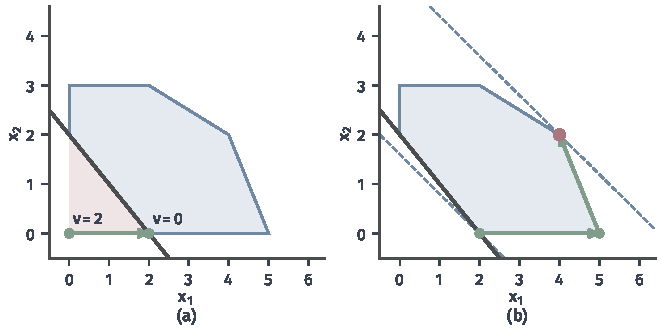
\includegraphics[width=112mm]{figures/05-optimization/01-linear-programming/matplotlib/simplex-two-phase-path/figure.pdf}
 \caption{两阶段法的路径。深灰粗线是合同约束$x_1+x_2=2$，浅蓝是原问题的可行域，它不含原点。(a)~第一阶段：从不可行的原点出发（红色浅底是违约区），沿$x_1$轴走到人工变量$v=x_7$降为零的点。(b)~第二阶段：从$(2,0)$出发，用原目标走到红色的最优点，蓝色虚线是利润$8$和$26$的等值线。}
 \label{fig:simplex-two-phase-path}
\end{BookInlineFigure}

\paragraph{第一阶段判定不可行}
把合同改成$x_1+x_2\geq7$。第一阶段从$\phi=7$开始，三轮的基和人工变量值为
\[
 \begin{aligned}
 B^{(0)}&=(3,4,5,7),& x_7&=7,\\
 B^{(1)}&=(3,1,5,7),& x_7&=2,\\
 B^{(2)}&=(2,1,5,7),& x_7&=1.
 \end{aligned}
\]
第$2$轮的对偶候选和约化成本是
\[
 \bm{y}=\Bigl(-\frac13,-\frac13,0,1\Bigr)^\top,\qquad
 s_3=\frac13,\quad s_4=\frac13,\quad s_6=1.
\]
全部非负而$\phi^\star=1>0$，原问题不可行。

证书$\bm{y}$可以翻译成一句平常的话。原料和工时两个约束各乘$\frac13$相加，得到$x_1+x_2\leq6$，这与$x_1+x_2\geq7$矛盾，差额正好是$\phi^\star=1$。图~\ref{fig:simplex-phase-one-infeasible}中，第一阶段把点推到离合同线最近的顶点，停在那里，仍差$1$。

\begin{BookInlineFigure}
 \centering
 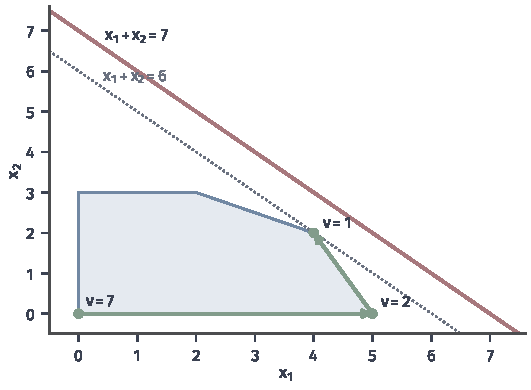
\includegraphics[width=90mm]{figures/05-optimization/01-linear-programming/matplotlib/simplex-phase-one-infeasible/figure.pdf}
 \caption{合同要求提高到$x_1+x_2\geq7$时的第一阶段。红线是合同边界，点线$x_1+x_2=6$是资源约束组合出的上限，两者之间没有可行点。绿色路径沿资源多边形的边界推进，人工变量$v$依次取$7,2,1$，在第一阶段最优点停在$v=1$。}
 \label{fig:simplex-phase-one-infeasible}
\end{BookInlineFigure}

\paragraph{基中残留的人工变量}
$\phi^\star=0$时，人工变量的值全为零，但可能有个别人工变量仍在基中，取值为零。第二阶段不能直接开始，否则人工变量可能在后续换基中重新变正。设它位于基的第$r$个位置，定义该行的系数
\begin{equation}
 \bm{\rho}=\bm{A}_B^{-\top}\bm{e}_r,\qquad \bar{a}_{r,j}=\bm{\rho}^\top\bm{a}_j,
 \label{eq:simplex-row-coefficients}
\end{equation}
其中$\bm{e}_r$是第$r$个坐标向量，$\bar{a}_{r,j}$就是把$\bm{a}_j$用基表示时第$r$个分量。分两种情况处理。

\begin{itemize}
 \item 存在原变量$x_j$（$j\in N$）使$\bar{a}_{r,j}\neq0$。把$x_j$换入第$r$个位置。由于该位置的值是零，步长为零，其他变量不变，符号不必为正。
 \item 对所有原变量都有$\bar{a}_{r,j}=0$。此时$\bm{\rho}^\top\bm{A}=\bm{0}^\top$，$\bm{\rho}\neq\bm{0}$，说明这一行是其余行的线性组合，是冗余等式，可以连同该人工变量一起删去。
\end{itemize}

第二种情况也说明，第~\ref{chap:linear-programming}章假定$\bm{A}$满行秩并不需要预先检查，第一阶段顺带就发现了冗余行。下面的例子展示两种情况。

\begin{example}[换出与删行]
 \label{ex:simplex-residual-artificial}
 考虑约束$x_1+x_2+x_3=2$，$2x_1+\omega(x_2+x_3)=4$，$\bm{x}\geq\bm{0}$，其中$\omega$取$1$或$2$，人工变量是$x_4,x_5$。从基$(4,5)$出发，$x_1$的约化成本最负。比值都是$2$，并列时取下标小的$x_4$出基，得到基$(1,5)$和
 \[
  \bm{x}_B=(2,0)^\top,\qquad \phi=0,\qquad\bm{\rho}=(-2,1)^\top.
 \]
 $x_5$在基中取零。

 取$\omega=1$时，系数是$\bar{a}_{2,2}=\bar{a}_{2,3}=-1\neq0$，把$x_2$换入第$2$个位置，步长为零，基变为$(1,2)$。

 取$\omega=2$时，系数是$\bar{a}_{2,2}=\bar{a}_{2,3}=0$。第二行正是第一行的$2$倍，删去第二行和$x_5$，基变为$(1)$。
\end{example}

图~\ref{fig:simplex-phase-flow}把两阶段法的分支整理在一起。

\begin{BookInlineFigure}
 \centering
 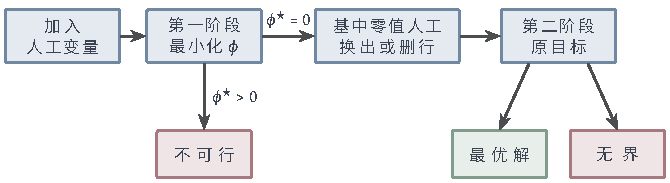
\includegraphics[width=112mm]{figures/05-optimization/01-linear-programming/tikz/simplex-phase-flow/figure.pdf}
 \caption{两阶段法的流程。第一阶段的最优值$\phi^\star$决定是否继续；基中取零的人工变量换出或连同冗余行删去后，第二阶段以原目标运行，以最优解或无界方向结束。红框是给出证书的否定结果，绿框是得到最优解。}
 \label{fig:simplex-phase-flow}
\end{BookInlineFigure}

\subsection{大M法}
\label{sec:simplex-big-m}

\paragraph{主要思想}
\term{大M法}（big-M method）把两个阶段合成一个问题，在目标中给人工变量定一个极高的单价：
\begin{equation}
 \min_{\bm{x},\bm{v}}\ \bm{c}^\top\bm{x}+M\,\bm{1}^\top\bm{v}
 \quad\text{s.t.}\quad
 \bm{A}\bm{x}+\bm{v}=\bm{b},\quad\bm{x}\geq\bm{0},\quad\bm{v}\geq\bm{0}.
 \label{eq:simplex-big-m}
\end{equation}
把$M$当作一个比任何数都大的符号来计算，约化成本就是形如$\beta+\gamma M$的式子，比较大小时先比$\gamma$，再比$\beta$。这样，只要还能减少人工变量，算法就不会先去改善原目标，排除人工变量自动享有优先权。

例中第$0$轮的对偶候选和约化成本是
\[
 \bm{y}=(0,0,0,M)^\top,\quad s_1=-4-M,\quad s_2=-5-M,\quad s_6=M.
\]
$s_1,s_2$里$M$的系数相同，再比常数项，$s_2$更负，$x_2$入基。此后各轮的数据在表~\ref{tab:simplex-big-m-rounds}中，路径见图~\ref{fig:simplex-big-m}(a)。第$0$轮换基后人工变量已经出基，接下来就是用原目标继续。

\begin{BookInlineTable}
 \centering
 \begin{tabular}{cccc}
  \toprule
  $t$ & $B^{(t)}$ & $(x_1,x_2)$ & 负的约化成本（入基）\\
  \midrule
  $0$ & $(3,4,5,7)$ & $(0,0)$ & $s_2=-5-M$，$s_1=-4-M$\\
  $1$ & $(3,4,5,2)$ & $(0,2)$ & $s_6=-5$\\
  $2$ & $(3,4,6,2)$ & $(0,3)$ & $s_1=-4$\\
  $3$ & $(1,4,6,2)$ & $(2,3)$ & $s_5=-3$\\
  $4$ & $(1,5,6,2)$ & $(4,2)$ & 无，停止\\
  \bottomrule
 \end{tabular}
 \caption{符号化大M法的各轮数据。}
 \label{tab:simplex-big-m-rounds}
\end{BookInlineTable}

\paragraph{有限的$M$要多大}
实际计算若取一个具体的数$M$，就必须问它够不够大。下面的定理给出精确的条件。

\begin{theorem}[有限惩罚的充分条件]
 \label{thm:simplex-finite-penalty}
 设标准型~\eqref{eq:simplex-standard-form}有最优解，最优值为$p^\star$，$\bm{y}^\star$是一个对偶最优解。若
 \begin{equation}
  M>\max_i\,y_i^\star,
  \label{eq:simplex-big-m-threshold}
 \end{equation}
 其中$i$取遍带人工变量的行，则问题~\eqref{eq:simplex-big-m}的最优值等于$p^\star$，并且它的每个最优解都满足$\bm{v}=\bm{0}$，其$\bm{x}$部分是原问题的最优解。
\end{theorem}

\begin{proof}
 为简洁起见设每行都有人工变量，其余情形只需令相应$v_i=0$。任取问题~\eqref{eq:simplex-big-m}的可行点$(\bm{x},\bm{v})$，记对偶松弛为$\bm{s}^\star\geq\bm{0}$，它满足$\bm{c}=\bm{s}^\star+\bm{A}^\top\bm{y}^\star$。把$\bm{c}$代换掉，并用$\bm{A}\bm{x}=\bm{b}-\bm{v}$，得到
 \[
  \bm{c}^\top\bm{x}
  =(\bm{s}^\star)^\top\bm{x}+(\bm{y}^\star)^\top\bm{A}\bm{x}
  \geq(\bm{y}^\star)^\top\bm{b}-(\bm{y}^\star)^\top\bm{v}.
 \]
 由强对偶，$\bm{b}^\top\bm{y}^\star=p^\star$，于是两边加上$M\bm{1}^\top\bm{v}$后，
 \[
  \bm{c}^\top\bm{x}+M\bm{1}^\top\bm{v}
  \geq p^\star+\sum_i(M-y_i^\star)v_i\geq p^\star.
 \]
 原问题的最优解配上$\bm{v}=\bm{0}$可行且取到$p^\star$，所以最优值是$p^\star$。若某个最优解有$v_i>0$，由式~\eqref{eq:simplex-big-m-threshold}上面最后一个不等号严格成立，与最优值为$p^\star$矛盾，所以$\bm{v}=\bm{0}$。此时$\bm{x}$可行且目标为$p^\star$，是原问题的最优解。
\end{proof}

门槛是对偶价格，这很合理：$y_i^\star$是放松第$i$条约束一单位时目标能下降多少，$M$是违反一单位约束要付的罚款。罚款高过这个收益，违约才不划算。

这个门槛取决于事先并不知道的$\bm{y}^\star$。把工厂的目标换成最小化成本$2x_1+3x_2$，合同约束就变成活动约束，最优解是$(2,0)$，对偶分量$y_4^\star=2$。图~\ref{fig:simplex-big-m}(b)对每个$M$精确求解，$M<2$时最优解干脆不生产，留着$v=2$付罚款，$M>2$时才回到真正的解。

\begin{BookInlineFigure}
 \centering
 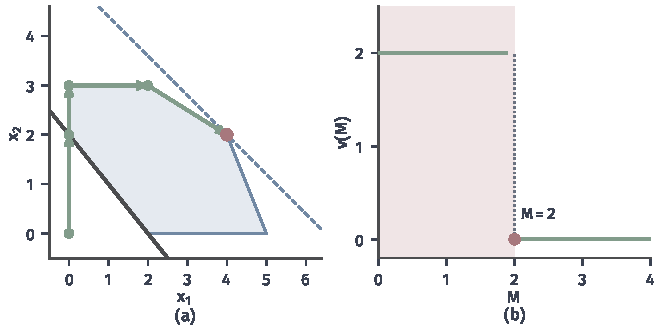
\includegraphics[width=112mm]{figures/05-optimization/01-linear-programming/matplotlib/simplex-big-m/figure.pdf}
 \caption{大M法。(a)~符号化大M在资源配置问题上的路径（绿色），第一步消去人工变量到达$(0,2)$，其后沿边界到最优点。(b)~目标$2x_1+3x_2+Mv$在不同有限$M$下的最优人工变量值$v(M)$：红色浅底的$M<2$区间内罚款不足，解停留在$v=2$；$M=2$时两种解并列（点线）；$M>2$时$v=0$。}
 \label{fig:simplex-big-m}
\end{BookInlineFigure}

$M$也不能随意取大。在双精度浮点数中，$10^{17}$附近相邻两个可表示数相差$16$，于是
\[
 -4-10^{17}\quad\text{和}\quad-5-10^{17}
\]
舍入后是同一个数，$c_1=-4$与$c_2=-5$的差别被抹掉，定价失去依据。系数相差过于悬殊还会使基矩阵病态。所以有限$M$不能靠“取一个很大的常数”得到保证；另外，若某个有限$M$的解有$v\neq\bm{0}$，也分不清是$M$不够大还是原问题不可行。

表~\ref{tab:simplex-two-phase-vs-big-m}对照了两种做法。

\begin{BookInlineTable}
 \centering
 \begin{tabular}{lll}
  \toprule
  & 两阶段法 & 大M法\\
  \midrule
  目标 & 先最小化$\bm{1}^\top\bm{v}$，再用$\bm{c}$ & 同时用$\bm{c}+M$惩罚\\
  不可行判定 & $\phi^\star>0$ & 符号化时$\bm{v}$不能消去\\
  参数 & 无 & 需要符号或足够大的$M$\\
  数值风险 & 无额外系数 & $M$过大使尺度恶化\\
  \bottomrule
 \end{tabular}
 \caption{两阶段法与大M法的对照。}
 \label{tab:simplex-two-phase-vs-big-m}
\end{BookInlineTable}

\section{退化的处理}
\label{sec:simplex-degeneracy}

定理~\ref{thm:simplex-finite-nondegenerate}的有限终止依赖一个假设：每次换基都能真正走出去。本节研究这个假设不成立时算法会发生什么，以及怎样修补。

\paragraph{同一个顶点，不同的基}
把工厂的工时从$10$改成$7$，三条约束边界就同时经过点$(2,3)$，如图~\ref{fig:simplex-degenerate-vertex}(a)所示。二维平面上确定一个点只需要两条线，这里却有三条，选哪两条都行。对应到代数上，这个点的$x_3=x_4=x_5=0$，三个变量中必须有一个留在基中，取值为零。这就是退化：一个基本可行解有基变量取零，同一个点可以对应多个基。

\begin{BookInlineFigure}
 \centering
 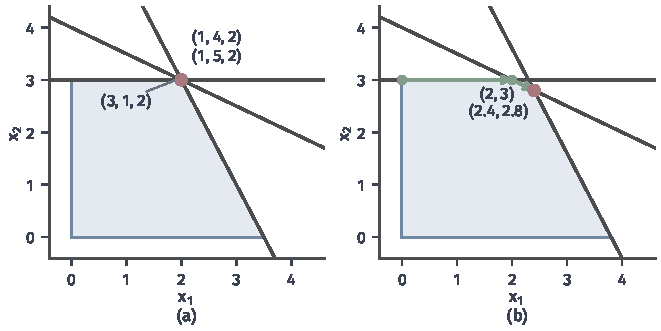
\includegraphics[width=112mm]{figures/05-optimization/01-linear-programming/matplotlib/simplex-degenerate-vertex/figure.pdf}
 \caption{退化顶点及其扰动。(a)~工时取$7$时三条约束边界（深灰）交于红点$(2,3)$，旁边的三元组是对应这同一个点的三个基。(b)~把工时夸张地增大到$7.6$后，这个顶点分裂成$(2,3)$和$(2.4,2.8)$两个相邻顶点，绿色路径多走一条真实的短边，每步都有实际移动。}
 \label{fig:simplex-degenerate-vertex}
\end{BookInlineFigure}

\paragraph{不移动的换基}
从基$(3,4,5)$开始运行Dantzig规则，前一轮与之前相同，$x_2$入基，点到$(0,3)$，基是$(3,4,2)$，$\bm{x}_B=(2,4,3)^\top$。下一轮$x_1$入基，$\bm{u}=(1,2,0)^\top$，两个比值并列：
\[
 \frac{2}{1}=2,\qquad \frac{4}{2}=2.
\]
这里的并列正是退化的来源：两个基变量同时降到零，只有一个能出基，另一个留下来取零。按下标小的规则，$x_3$出基，得到
\[
 B=(1,4,2),\qquad \bm{x}_B=(2,0,3)^\top,\qquad f=-23,
\]
点到达$(2,3)$。

此时的对偶候选和约化成本是
\[
 \bm{y}=(-4,0,3)^\top,\qquad s_3=4,\qquad s_5=-3.
\]
$s_5<0$，判别说还不能停。$x_5$入基，$\bm{u}=(-2,3,1)^\top$，比值是
\[
 \frac{x_4}{u_2}=\frac{0}{3}=0,\qquad \frac{x_2}{u_3}=\frac{3}{1}=3.
\]
步长$\alpha=0$，基变成$(1,5,2)$，点和目标都没变。新基的对偶候选和约化成本是
\[
 \bm{y}=(-2,-1,0)^\top,\qquad s_3=2,\qquad s_4=1,
\]
全部非负，算法才停下。

其实$(2,3)$早已是最优点，这一轮换基只是把基换成能出示证书的那一个。如果上一轮并列时让$x_4$出基，就直接得到基$(3,1,2)$，此时$\bm{y}=(0,-2,-3)^\top$，$s_4=2$，$s_5=3$，立即停止。这说明两点：退化基上$s_j<0$并不表示当前点不是最优；证书依赖基，同一个最优点上有的基能给出证书，有的基不能。

\paragraph{循环}
既然目标可以不下降，“每步都变好”的论证就失效了，算法可能在一组基之间兜圈子，这称为\term{循环}（cycling）。下面是一个有三行四个决策变量的例子，$x_5,x_6,x_7$是松弛变量：
\begin{equation}
 \begin{aligned}
 \min\quad & -10x_1+57x_2+9x_3+24x_4\\
 \text{s.t.}\quad & \tfrac12x_1-\tfrac{11}{2}x_2-\tfrac52x_3+9x_4+x_5=0,\\
 & \tfrac12x_1-\tfrac32x_2-\tfrac12x_3+x_4+x_6=0,\\
 & x_1+x_7=1,\qquad \bm{x}\geq\bm{0}.
 \end{aligned}
 \label{eq:simplex-cycling-example}
\end{equation}
用Dantzig规则，比值并列时取下标最小者，从基$(5,6,7)$出发，得到表~\ref{tab:simplex-cycling-rounds}的序列。每一步都有负的约化成本，每一步的步长都是零，第$6$步回到起点。

\begin{BookInlineTable}
 \centering
 \begin{tabular}{ccccc}
  \toprule
  $t$ & $B^{(t)}$ & 入基 & 约化成本 & 出基\\
  \midrule
  $0$ & $(5,6,7)$ & $x_1$ & $-10$ & $x_5$\\
  $1$ & $(1,6,7)$ & $x_2$ & $-53$ & $x_6$\\
  $2$ & $(1,2,7)$ & $x_3$ & $-29/2$ & $x_1$\\
  $3$ & $(3,2,7)$ & $x_4$ & $-18$ & $x_2$\\
  $4$ & $(3,4,7)$ & $x_5$ & $-21/2$ & $x_3$\\
  $5$ & $(5,4,7)$ & $x_6$ & $-24$ & $x_4$\\
  $6$ & $(5,6,7)$ & 回到第$0$轮 & & \\
  \bottomrule
 \end{tabular}
 \caption{问题~\eqref{eq:simplex-cycling-example}在Dantzig规则下的循环。}
 \label{tab:simplex-cycling-rounds}
\end{BookInlineTable}

图~\ref{fig:simplex-cycle-bases}把这六个基画成一个环。这个环上$\bm{x}$从未变化，所以只看目标值的话，看不出算法在做什么。

\begin{BookInlineFigure}
 \centering
 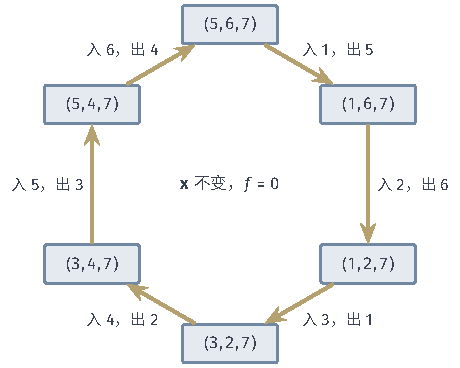
\includegraphics[width=78mm]{figures/05-optimization/01-linear-programming/tikz/simplex-cycle-bases/figure.pdf}
 \caption{问题~\eqref{eq:simplex-cycling-example}的六个基组成的循环。方框是基，黄色箭头是Dantzig规则下的一次换基，箭头旁写明入基和出基下标。整个环上$\bm{x}$和目标值都不变。}
 \label{fig:simplex-cycle-bases}
\end{BookInlineFigure}

\paragraph{Bland规则}
要打破循环，只需把“选哪一个”的自由度用一条固定的规则收走。\term{Bland规则}（Bland's rule）规定：入基变量取所有$s_j<0$中下标最小的；比值检验并列时，出基变量取下标最小的\scite{math-bland1977finite}。

\begin{theorem}[Bland规则的有限终止]
 \label{thm:simplex-bland}
 在精确算术下，使用Bland规则的单纯形法不会循环，因而经过有限次换基后停止。
\end{theorem}

\begin{proof}
 假设出现循环。目标值不增，循环中目标必须保持不变，所以每一步的步长都是零，$\bm{x}$在整个循环中不变，记为$\bar{\bm{x}}$。

 称循环中曾经入基的下标为活跃下标，活跃下标也必定曾经出基。活跃下标在某个基中非基，所以对应的$\bar{x}_j=0$。设$k$是最大的活跃下标。取循环中$k$将要出基的一个基$B$，此时入基的是活跃下标$q<k$。再取循环中$k$将要入基的一个基$B'$，其约化成本记为$\bm{s}'$，对偶候选记为$\bm{y}'$。

 由基$B$和入基$q$按式~\eqref{eq:simplex-direction}构造方向$\bm{d}$，它满足
 \[
  \bm{A}\bm{d}=\bm{0},\qquad \bm{c}^\top\bm{d}=s_q<0.
 \]
 用$\bm{s}'=\bm{c}-\bm{A}^\top\bm{y}'$，得到
 \[
  (\bm{s}')^\top\bm{d}=\bm{c}^\top\bm{d}-(\bm{y}')^\top\bm{A}\bm{d}=s_q<0.
 \]
 因此存在下标$j$使$s'_jd_j<0$。

 这个$j$满足$j\notin B'$，因为$B'$的基变量$s'_j=0$；同时$d_j\neq0$，故$j\in B$或$j=q$。两种情况下$j$都在循环中某一时刻属于基或正要入基，而在$B'$非基，所以$j$是活跃下标，$j\leq k$。

 下面排除$j=k$。$k$在$B$中将要出基，说明$u_k>0$，$d_k<0$；而$k$在$B'$中将要入基，说明$s'_k<0$。于是$s'_kd_k>0$，所以$j\neq k$，只能$j<k$。

 Bland规则在$B'$选了$k$入基，这说明比$k$小的下标都没有负的约化成本，所以$s'_j\geq0$，结合$s'_jd_j<0$得到$s'_j>0$，$d_j<0$。特别地$j\neq q$，所以$j\in B$，且$u_j=-d_j>0$。又$j$活跃，$\bar{x}_j=0$，于是$j$的比值是$0$，与$k$的比值并列。$j<k$却没有被选中出基，这与Bland规则矛盾。

 不循环意味着基不重复，基的个数有限，所以换基只能进行有限次。
\end{proof}

证明的结构值得留意：用最大的活跃下标构造一个对偶上的矛盾，正是“取下标最小”这个规则使矛盾成立。这个规则的作用是保证有限，不是追求速度，它常常比Dantzig规则走更多步。

回到问题~\eqref{eq:simplex-cycling-example}，Bland规则的前$5$步与表~\ref{tab:simplex-cycling-rounds}相同。第$5$轮基是$(5,4,7)$，约化成本$s_1=-22$，$s_6=-24$。Dantzig规则选$s_6$回到起点，Bland规则选下标小的$x_1$，走出了循环。再换一次基后，$x_3$入基时唯一的比值来自$x_7$，$\alpha=1$，得到
\[
 \bm{x}=(1,0,1,0,2,0,0)^\top,\qquad f=-1,
\]
约化成本全部非负。图~\ref{fig:simplex-cycling-objective}对比了两种规则的目标值。

\begin{BookInlineFigure}
 \centering
 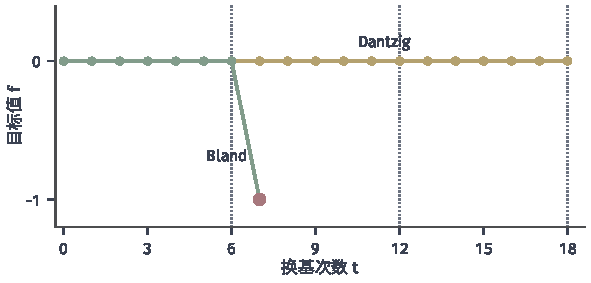
\includegraphics[width=100mm]{figures/05-optimization/01-linear-programming/matplotlib/simplex-cycling-objective/figure.pdf}
 \caption{问题~\eqref{eq:simplex-cycling-example}上两种规则的目标值。黄线是Dantzig规则，目标值恒为$0$，竖直点线标出每$6$步回到起始基；绿线是Bland规则，$6$次零步之后第$7$次换基走到红色的最优点，$f=-1$。}
 \label{fig:simplex-cycling-objective}
\end{BookInlineFigure}

\paragraph{字典序规则}
图~\ref{fig:simplex-degenerate-vertex}(b)提示了另一条路：既然麻烦来自几条约束恰好相交于一点，就把右端轻轻推开，让退化顶点裂成几个相距很近的普通顶点。把右端换成
\[
 \bm{b}+(\epsilon,\epsilon^2,\ldots,\epsilon^m)^\top,
\]
其中$\epsilon>0$充分小，比值并列就不会发生，每步都有严格的下降。

\term{字典序规则}（lexicographic rule）把这个想法做成不需要真的取$\epsilon$的规则：比值并列时，比较各并列行的向量$[\bar{x}_{B(i)},(\bm{A}_B^{-1})_{i,:}]/u_i$，取字典序最小者出基。它的作用等同于对无穷小的扰动做比值检验。证明需要跟踪各行字典序为正这一性质，并说明每次换基使目标行严格字典序下降，读者可查阅线性规划专著\scite{math-bertsimas1997linear}。结论同样是：在精确算术下不循环，有限终止。

两种规则的保证都建立在精确算术之上。浮点计算里，“恰好是零”没有意义，比值并列要用容差判断，舍入误差也会把退化基上的零扰动成微小的正负数。所以实现时除了防循环的规则，还要在最后重新核查可行性和约化成本，第~\ref{sec:simplex-revised}节将说明怎样做。

\section{修正单纯形法}
\label{sec:simplex-revised}

前面把算法写成了矩阵公式，每轮都出现$\bm{A}_B^{-1}$。接下来要弄清：真正计算时应该保存什么，每轮要做多少运算？

\paragraph{完整的单纯形表}
最直接的办法是把所有非基变量的表示都算出来，存成一张表。\term{单纯形表}（simplex tableau）的主体是$\bm{A}_B^{-1}[\bm{b}\ \ \bm{A}]$，再加一行约化成本。例中第$2$轮的基是$(1,4,2)$，表~\ref{tab:simplex-tableau}的上半部分就是这张表，每一列都是对应$\bm{a}_j$在当前基下的表示，$u$和$\bar{x}_B$都可以直接读出。

换基就是对这张表做一次Gauss--Jordan消元，主元取在出基行和入基列的交点。例中主元是$x_4$行$x_5$列的$3$。把该行除以$3$，再用它消去$x_5$列的其他元素，就得到下半部分，也就是第$3$轮的表。

\begin{BookInlineTable}
 \centering
 \begin{tabular}{crrrrrr}
  \toprule
  基 & $\bar{x}$ & $x_1$ & $x_2$ & $x_3$ & $x_4$ & $x_5$\\
  \midrule
  $x_1$ & $2$ & $1$ & $0$ & $1$ & $0$ & $-2$\\
  $x_4$ & $3$ & $0$ & $0$ & $-2$ & $1$ & $3$\\
  $x_2$ & $3$ & $0$ & $1$ & $0$ & $0$ & $1$\\
  $\bm{s}$ & $23$ & $0$ & $0$ & $4$ & $0$ & $-3$\\
  \midrule
  $x_1$ & $4$ & $1$ & $0$ & $-1/3$ & $2/3$ & $0$\\
  $x_5$ & $1$ & $0$ & $0$ & $-2/3$ & $1/3$ & $1$\\
  $x_2$ & $2$ & $0$ & $1$ & $2/3$ & $-1/3$ & $0$\\
  $\bm{s}$ & $26$ & $0$ & $0$ & $2$ & $1$ & $0$\\
  \bottomrule
 \end{tabular}
 \caption{资源配置问题第$2$轮（上）和第$3$轮（下）的单纯形表。第二列是基变量取值，$\bm{s}$行第二列是利润$-f$，其余是约化成本。}
 \label{tab:simplex-tableau}
\end{BookInlineTable}

这张表手算方便，但代价不小：每轮要更新大约$(m+1)(n+1)$个数，无论这一轮用到多少。而且$\bm{A}$稀疏时，$\bm{A}_B^{-1}\bm{A}$通常是稠密的，存储量也不可接受。

\paragraph{每轮真正需要什么}
回头看第~\ref{sec:simplex-basis-exchange}节的计算步骤，一轮只用到四样东西：解一次$\bm{A}_B^\top\bm{y}=\bm{c}_B$，用$\bm{y}$和$\bm{A}$的非基列做内积定价，对入基列解一次$\bm{A}_B\bm{u}=\bm{a}_q$，再做比值检验。表中其他列的表示从未被使用。\term{修正单纯形法}（revised simplex method）因此只维护基矩阵的因子，其余的量需要时再算。一轮的数据流如图~\ref{fig:simplex-revised-flow}所示。

\begin{BookInlineFigure}
 \centering
 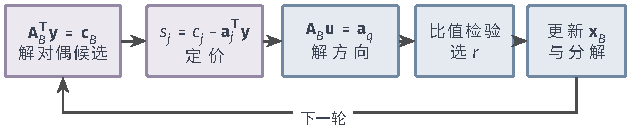
\includegraphics[width=107mm]{figures/05-optimization/01-linear-programming/tikz/simplex-revised-flow/figure.pdf}
 \caption{修正单纯形法一轮的数据流。紫色框处理对偶量：解$\bm{A}_B^\top\bm{y}=\bm{c}_B$得到对偶候选，再对非基列定价。蓝色框处理原始量：解$\bm{A}_B\bm{u}=\bm{a}_q$，比值检验选出基位置，更新基变量和基矩阵的因子。}
 \label{fig:simplex-revised-flow}
\end{BookInlineFigure}

\paragraph{基矩阵逆的更新}
相邻两轮的基矩阵只差一列，无需重新分解。设新基$B'$把第$r$列换成$\bm{a}_q$。由$\bm{a}_q=\bm{A}_B\bm{u}$，新基矩阵可以写成
\[
 \bm{A}_{B'}=\bm{A}_B\bm{F},
\]
其中$\bm{F}$是把单位矩阵第$r$列换成$\bm{u}$的矩阵。两边求逆，只需要$\bm{F}$的逆，它仍是单位矩阵只改第$r$列的形状：
\begin{equation}
 \bm{A}_{B'}^{-1}=\bm{E}\bm{A}_B^{-1},\qquad
 \bm{E}_{:,r}=\bm{\eta},\qquad
 \eta_i=
 \begin{cases}
  -u_i/u_r,& i\neq r,\\
  1/u_r,& i=r.
 \end{cases}
 \label{eq:simplex-eta-update}
\end{equation}
这样的$\bm{E}$只需保存一列，称为eta矩阵。

例中从第$2$轮到第$3$轮，$\bm{u}=(-2,3,1)^\top$，$r=2$，于是
\[
 \bm{E}=\begin{bmatrix}1&2/3&0\\0&1/3&0\\0&-1/3&1\end{bmatrix}.
\]
第$2$轮的基矩阵逆左乘$\bm{E}$，就得到第$3$轮的基矩阵逆：
\begin{equation}
 \bm{A}_{B^{(3)}}^{-1}
 =\bm{E}\begin{bmatrix}1&0&-2\\-2&1&3\\0&0&1\end{bmatrix}
 =\begin{bmatrix}-1/3&2/3&0\\-2/3&1/3&1\\2/3&-1/3&0\end{bmatrix}.
 \label{eq:simplex-final-inverse}
\end{equation}
这个矩阵的第$r$行就是式~\eqref{eq:simplex-row-coefficients}中的$\bm{\rho}$，后两节会反复用到它。

\paragraph{运算量的比较}
表~\ref{tab:simplex-implementation-costs}列出每轮的存储和运算。这里$\operatorname{nnz}(\cdot)$表示非零元个数。修正法的优势在$n\gg m$或$\bm{A}$稀疏时最明显：定价只碰$\bm{A}$的非零元，解方程只碰因子的非零元。

\begin{BookInlineTable}
 \centering
 \begin{tabular}{lll}
  \toprule
  实现方式 & 存储 & 每轮主要运算\\
  \midrule
  完整单纯形表 & $(m+1)(n+1)$ & 约$mn$次更新\\
  修正法，稠密逆 & $m^2$ & 约$m^2+\operatorname{nnz}(\bm{A})$\\
  修正法，LU加eta & 因子的非零元 & 两次三角回代加定价\\
  \bottomrule
 \end{tabular}
 \caption{单纯形法几种实现的每轮代价，均指量级。}
 \label{tab:simplex-implementation-costs}
\end{BookInlineTable}

\paragraph{稀疏性}
大规模问题的基矩阵往往非常稀疏，这时不应显式保存逆。图~\ref{fig:simplex-sparsity}是一个$40$阶三对角矩阵的例子。矩阵本身和它的LU因子都只有$118$个非零位置，而逆矩阵的$1600$个元素全部非零。实际软件保存基矩阵经过行列重排的LU分解，再累积一串eta矩阵，这也是用稀疏因子代替稠密逆的具体办法。重排的目的是减少分解过程中新产生的非零元；LU分解和三角回代的基本算法，可参考\BookChapterRef{chap:direct-linear-solvers}{卷二第12章“线性方程的直接求解”}。

\begin{BookInlineFigure}
 \centering
 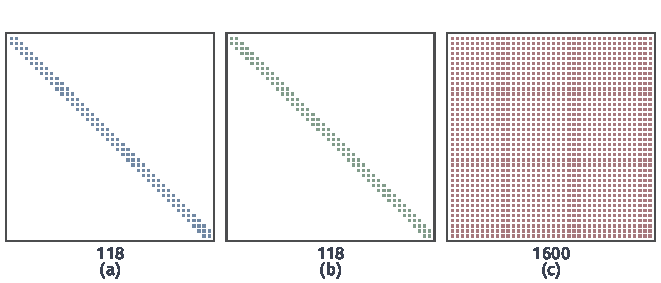
\includegraphics[width=112mm]{figures/05-optimization/01-linear-programming/matplotlib/simplex-sparsity/figure.pdf}
 \caption{$40$阶三对角基矩阵的非零结构，每个小点是一个非零元，图下的数字是非零元总数。(a)~矩阵本身。(b)~不选主元的LU因子合在一起，没有新增非零元。(c)~逆矩阵，全部$1600$个元素非零。}
 \label{fig:simplex-sparsity}
\end{BookInlineFigure}

\paragraph{舍入误差}
连续用eta矩阵更新，每一步都要除以$u_r$。若主元$u_r$很小，比如$10^{-12}$，$\bm{\eta}$的元素可达$10^{12}$量级，舍入误差被同比放大，并一直留在后续的所有计算里。图~\ref{fig:simplex-refactorization}是一个固定随机种子的实验：在$120$阶稠密随机基矩阵上连续换入随机列，比较选取不同主元的残差。总选最大的主元时残差始终在$10^{-13}$左右；总选合格主元中最小的那个时，残差上升好几个数量级，定期重新分解能把它拉回来，但只要继续用小主元，残差又会很快上升。

\begin{BookInlineFigure}
 \centering
 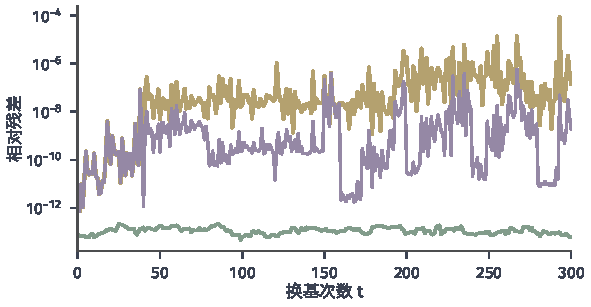
\includegraphics[width=100mm]{figures/05-optimization/01-linear-programming/matplotlib/simplex-refactorization/figure.pdf}
 \caption{用更新后的逆求$\bm{x}_B$时的相对残差$\lVert\bm{A}_B\bm{x}_B-\bm{b}\rVert_2/\lVert\bm{b}\rVert_2$，随机种子固定，矩阵阶数$120$。绿线每步选最大主元且不重分解；黄线每步选$\lvert u_r\rvert>10^{-4}$中最小的主元且不重分解；紫线的选法同黄线，但每$40$次换基重新计算一次逆。}
 \label{fig:simplex-refactorization}
\end{BookInlineFigure}

实验提示了实现时的几条具体做法。比值检验并列或接近并列时，优先选$\lvert u_r\rvert$大的主元，低于主元容差的不选。累积若干个eta矩阵后，重新分解$\bm{A}_B$，用新因子重算$\bm{x}_B,\bm{y},\bm{s}$。

浮点数下的“非负”也只能在容差内判断。常见的可行性容差在$10^{-9}$到$10^{-6}$之间，即接受$x_j\geq-\varepsilon$，约化成本用同样的方式判断。因此算法报告“最优”的含义是：在给定容差下，$\bm{A}\bm{x}=\bm{b}$的残差、$\bm{x}$的负部和$\bm{s}$的负部都足够小。收尾时应该用新的分解重算一遍这三个量，并做必要的尺度还原，因为这些容差是在内部缩放后的问题上判断的，换回原单位后需要另行核查。

\section{对偶单纯形法}
\label{sec:simplex-dual}

工厂解完问题后，资源情况变了：原料增加到$13$，工时骤减到$2$，设备增加到$4$。这就需要回答：手里的最优基还能怎样利用，而不必从头求解？

\paragraph{基的两种可行性}
约化成本只依赖$\bm{c}$和基，与$\bm{b}$无关。所以右端变化后，原来的最优基$(1,5,2)$依然满足$\bm{s}\geq\bm{0}$，也就是对偶可行。受影响的是基变量。用式~\eqref{eq:simplex-final-inverse}的逆矩阵计算，新的基变量是
\[
 \bm{x}_B=\bm{A}_B^{-1}\begin{bmatrix}13\\2\\4\end{bmatrix}=\begin{bmatrix}-3\\-4\\8\end{bmatrix}.
\]
基失去了原始可行性，而对偶可行性完好。这正好与上一节相反：原始单纯形法保持$\bm{x}_B\geq\bm{0}$，逐步争取$\bm{s}\geq\bm{0}$；现在我们手里是$\bm{s}\geq\bm{0}$，需要逐步争取$\bm{x}_B\geq\bm{0}$。\term{对偶单纯形法}（dual simplex method）做的就是这件事。

\paragraph{主要思想}
选一个$\bar{x}_{B(r)}<0$的位置，让这个基变量出基。写出第$r$行，由式~\eqref{eq:simplex-basic-form}和式~\eqref{eq:simplex-row-coefficients}，每个满足等式的点都有
\begin{equation}
 x_{B(r)}+\sum_{j\in N}\bar{a}_{r,j}x_j=\bar{x}_{B(r)}<0.
 \label{eq:simplex-dual-row}
\end{equation}
要把$x_{B(r)}$抬到零，必须让某个$\bar{a}_{r,j}<0$的非基变量变大。候选可能有好几个，选哪一个由对偶可行性决定。

换到对偶的角度看。沿方向$\bm{\rho}$改变对偶变量，令$\bm{y}(\tau)=\bm{y}-\tau\bm{\rho}$，$\tau\geq0$。第一，对偶目标增大，这是我们想要的：
\[
 \bm{b}^\top\bm{y}(\tau)=\bm{b}^\top\bm{y}-\tau\,\bar{x}_{B(r)},
\]
这里用到了$\bm{\rho}^\top\bm{b}=\bar{x}_{B(r)}$。第二，约化成本线性变化：
\begin{equation}
 s_j(\tau)=c_j-\bm{a}_j^\top\bm{y}+\tau\,\bm{a}_j^\top\bm{\rho}=s_j+\tau\,\bar{a}_{r,j}.
 \label{eq:simplex-dual-reduced-cost}
\end{equation}
其他基变量的$\bar{a}_{r,j}=0$，它们的约化成本保持为零；第$r$个基变量的$\bar{a}_{r,j}=1$，约化成本变为$\tau\geq0$。非基变量中$\bar{a}_{r,j}\geq0$的不会变差，$\bar{a}_{r,j}<0$的会下降，下降到零时就必须停止。这就是对偶的比值检验：
\begin{equation}
 \tau^\star=\min_{j\in N:\,\bar{a}_{r,j}<0}\frac{s_j}{-\bar{a}_{r,j}}.
 \label{eq:simplex-dual-ratio}
\end{equation}
取到最小值的$q$入基，它的约化成本恰好变成零，所有约化成本仍然非负。

对比原始比值检验：原始检验防止基变量变负，选最先碰零的基变量出基；对偶检验防止约化成本变负，选最先碰零的非基变量入基。两者结构完全对称。表~\ref{tab:simplex-primal-dual-comparison}列出这种对称。

\begin{BookInlineTable}
 \centering
 \begin{tabular}{lll}
  \toprule
  & 原始单纯形法 & 对偶单纯形法\\
  \midrule
  保持 & $\bm{x}_B\geq\bm{0}$ & $\bm{s}\geq\bm{0}$\\
  争取 & $\bm{s}\geq\bm{0}$ & $\bm{x}_B\geq\bm{0}$\\
  先选 & $s_q<0$，入基 & $\bar{x}_{B(r)}<0$，出基\\
  比值检验选 & 出基位置 & 入基下标\\
  目标值 & 单调下降 & 单调上升\\
  否定结论 & 无界 & 不可行\\
  \bottomrule
 \end{tabular}
 \caption{原始单纯形法与对偶单纯形法的对照。}
 \label{tab:simplex-primal-dual-comparison}
\end{BookInlineTable}

式~\eqref{eq:simplex-dual-row}也解释了没有候选时的结论。若所有$\bar{a}_{r,j}\geq0$，式~\eqref{eq:simplex-dual-row}左端对任何$\bm{x}\geq\bm{0}$都非负，右端却是负数，所以无解。

\begin{theorem}[对偶单纯形法的不可行证书]
 \label{thm:simplex-dual-infeasible}
 设$\bar{x}_{B(r)}<0$，且所有$j\in N$都有$\bar{a}_{r,j}\geq0$，则$\bm{A}\bm{x}=\bm{b}$，$\bm{x}\geq\bm{0}$无解，$\bm{\rho}$满足
 \begin{equation}
  \bm{A}^\top\bm{\rho}\geq\bm{0},\qquad \bm{b}^\top\bm{\rho}=\bar{x}_{B(r)}<0.
  \label{eq:simplex-dual-certificate}
 \end{equation}
\end{theorem}

\begin{proof}
 基列的$\bm{\rho}^\top\bm{a}_j$是$0$或$1$，非基列的$\bm{\rho}^\top\bm{a}_j=\bar{a}_{r,j}\geq0$，所以$\bm{A}^\top\bm{\rho}\geq\bm{0}$；$\bm{b}^\top\bm{\rho}$是$\bm{A}_B^{-1}\bm{b}$的第$r$个分量。若有可行点$\bm{x}$，则
 \[
  0\leq\bm{x}^\top\bm{A}^\top\bm{\rho}=\bm{b}^\top\bm{\rho}<0,
 \]
 矛盾。
\end{proof}

\needspace{6\baselineskip}
\paragraph{变量}
沿用原始单纯形法的$B^{(t)},\bm{x}_B^{(t)},\bm{y}^{(t)},\bm{s}^{(t)},\bm{u}^{(t)}$，另增下面的量。
\begin{itemize}
 \item $r^{(t)}$：出基位置，$p^{(t)}=B^{(t)}(r^{(t)})$是出基下标。
 \item $\bm{\rho}^{(t)}\in\mathbb{R}^m$：$\bm{A}_B^{-\top}\bm{e}_r$；$\bar{a}_{r,j}^{(t)}$：第$r$行对第$j$列的系数。
 \item $\tau^{(t)}\geq0$：对偶步长；$q^{(t)}$：入基下标；$\alpha^{(t)}$：原始步长。
\end{itemize}

\paragraph{初始化}
需要一个对偶可行基。例中取原来的最优基，数据由式~\eqref{eq:simplex-resource-dual}和上面的计算得到：
\[
 B^{(0)}=(1,5,2),\qquad \bm{x}_B^{(0)}=(-3,-4,8)^\top,\qquad \bm{y}^{(0)}=(-2,-1,0)^\top.
\]
约化成本是$s_3=2$，$s_4=1$，对偶目标$\bm{b}^\top\bm{y}^{(0)}=-28$。这个$-28$比原问题的最优值低，它是新问题最优值的一个下界，算法要把它抬高。

\needspace{6\baselineskip}
\paragraph{每轮更新}
第$t$轮依次做下面几步。步骤后的“例中”是第$0$轮的数据。
\begin{enumerate}

 \item 判别。若$\bm{x}_B^{(t)}\geq\bm{0}$，停止，当前解最优。否则选负分量位置$r$出基，常取最负的。例中最负的是$x_5=-4$：
 \[
  r^{(0)}=2,\qquad p^{(0)}=5.
 \]

 \item 计算第$r$行。由式~\eqref{eq:simplex-row-coefficients}，例中取式~\eqref{eq:simplex-final-inverse}的第$2$行：
 \[
  \bm{\rho}^{(0)}=\Bigl(-\frac23,\frac13,1\Bigr)^\top,\qquad
  \bar{a}_{2,3}=-\frac23,\qquad \bar{a}_{2,4}=\frac13.
 \]

 \item 对偶比值检验。若所有$\bar{a}_{r,j}\geq0$，停止，按定理~\ref{thm:simplex-dual-infeasible}报告不可行。否则由式~\eqref{eq:simplex-dual-ratio}确定$\tau^{(t)}$和$q^{(t)}$。例中只有$x_3$是候选：
 \[
  \tau^{(0)}=\frac{2}{2/3}=3,\qquad q^{(0)}=3.
 \]

 \item 更新对偶量。沿$\bm{\rho}$移动，由式~\eqref{eq:simplex-dual-reduced-cost}更新约化成本：
 \begin{equation}
  \bm{y}^{(t+1)}=\bm{y}^{(t)}-\tau^{(t)}\bm{\rho}^{(t)},\qquad
  s_j^{(t+1)}=s_j^{(t)}+\tau^{(t)}\bar{a}_{r,j}^{(t)}.
  \label{eq:simplex-dual-update}
 \end{equation}
 例中
 \[
  \bm{y}^{(1)}=(0,-2,-3)^\top,\qquad s_4^{(1)}=1+3\cdot\frac13=2,\qquad s_5^{(1)}=3.
 \]

 \item 更新原始量。先求$\bm{u}^{(t)}=\bm{A}_B^{-1}\bm{a}_q$，取原始步长$\alpha^{(t)}=\bar{x}_{B(r)}/\bar{a}_{r,q}$，它是让第$r$个基变量恰好变成零的步长。其余基变量按式~\eqref{eq:simplex-primal-update}更新，第$r$个位置放$x_q=\alpha^{(t)}$。例中
 \[
  \bm{u}^{(0)}=\Bigl(-\frac13,-\frac23,\frac23\Bigr)^\top,\qquad
  \alpha^{(0)}=\frac{-4}{-2/3}=6.
 \]
 于是
 \[
  B^{(1)}=(1,3,2),\qquad \bm{x}_B^{(1)}=(-1,6,4)^\top,\qquad \bm{b}^\top\bm{y}^{(1)}=-16.
 \]
\end{enumerate}

例中第$1$轮只剩$x_1=-1$为负，所以$r=1$，$x_1$出基。第$1$行的系数和唯一的候选是
\[
 \bm{\rho}^{(1)}=\Bigl(0,\frac12,-\frac12\Bigr)^\top,\qquad
 \bar{a}_{1,4}=\frac12,\qquad \bar{a}_{1,5}=-\frac12,\qquad
 \tau^{(1)}=\frac{3}{1/2}=6.
\]
于是$x_5$入基，由式~\eqref{eq:simplex-dual-update}得到
\[
 \bm{y}^{(2)}=(0,-5,0)^\top,\qquad s_1^{(2)}=6,\qquad s_4^{(2)}=2+6\cdot\frac12=5.
\]
原始量的更新用
\[
 \bm{u}^{(1)}=\Bigl(-\frac12,-\frac32,1\Bigr)^\top,\qquad
 \alpha^{(1)}=\frac{-1}{-1/2}=2,
\]
更新后得到
\[
 B^{(2)}=(5,3,2),\qquad \bm{x}_B^{(2)}=(2,9,2)^\top,\qquad \bm{b}^\top\bm{y}^{(2)}=-10.
\]
第$2$轮$\bm{x}_B\geq\bm{0}$，算法停止。

\paragraph{最终得到}
新问题的最优解和最优值是
\[
 (x_1,x_2)=(0,2),\qquad p^\star=-10.
\]
工时只有$2$，全部给利润率更高的产品二最合算。对偶目标依次是$-28,-16,-10$，每一步增加$\tau\lvert\bar{x}_{B(r)}\rvert$，即$3\cdot4=12$和$6\cdot1=6$，它们一直是最优值的下界，到达时恰好等于最优值。这与第~\ref{sec:simplex-basis-exchange}节目标从上方下降的情形相反。

图~\ref{fig:simplex-dual-path}(a)显示了路径的特点：前两个点$(-3,8)$和$(-1,4)$都在可行域之外，它们是一系列“太便宜而不可能达到”的解，算法一步步向可行域靠拢，碰到可行域时恰好最优。

\begin{BookInlineFigure}
 \centering
 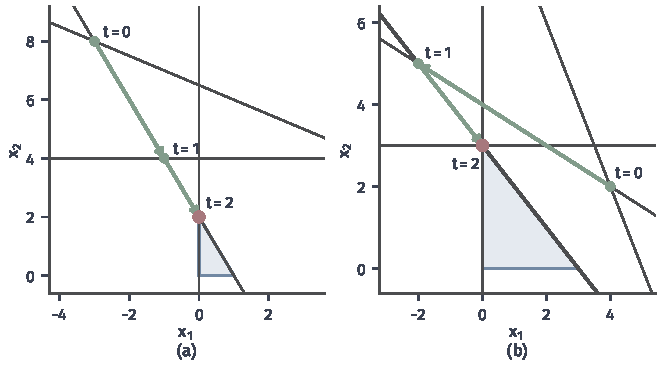
\includegraphics[width=112mm]{figures/05-optimization/01-linear-programming/matplotlib/simplex-dual-path/figure.pdf}
 \caption{对偶单纯形法在原始空间的路径（绿色），深灰线是约束边界，浅蓝是可行域，红点是最优解。(a)~右端变为$(13,2,4)$后，从不可行点$(-3,8)$经$(-1,4)$到$(0,2)$。(b)~新增约束$x_1+x_2\leq3$（粗线）后，从原最优点$(4,2)$经不可行点$(-2,5)$到$(0,3)$。}
 \label{fig:simplex-dual-path}
\end{BookInlineFigure}

\paragraph{新增约束与基的复用}
加入新约束是另一种常见的情形。给工厂加一条约束$x_1+x_2\leq3$，并引入松弛变量$x_6$。把$x_6$放入基，原最优基扩展成$(1,5,2,6)$。新基对偶可行，因为新列只增加一个取零的约化成本；只有$x_6$可能违反非负，这里$x_6=3-6=-3$。

第$0$轮$x_6$出基，第$4$行的系数和两个候选比值是
\[
 \bar{a}_{4,3}=-\frac13,\qquad \bar{a}_{4,4}=-\frac13,\qquad
 \frac{2}{1/3}=6,\qquad \frac{1}{1/3}=3.
\]
图~\ref{fig:simplex-dual-ratio}把这两个比值画成约化成本随$\tau$下降的直线，$s_4$先碰到零，所以$x_4$入基。再经一轮换基，$\bm{x}_B$全部非负，得到$(x_1,x_2)=(0,3)$，利润$15$。

\begin{BookInlineFigure}
 \centering
 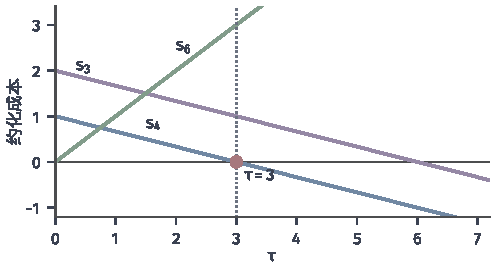
\includegraphics[width=84mm]{figures/05-optimization/01-linear-programming/matplotlib/simplex-dual-ratio/figure.pdf}
 \caption{新增约束后第$0$轮的对偶比值检验。三条直线是约化成本随对偶步长$\tau$的变化：$s_3=2-\tau/3$，$s_4=1-\tau/3$，$s_6=\tau$。红点是最先降到零的位置$\tau=3$，它决定入基变量$x_4$；$s_6$对应出基的$x_6$，只增不减。}
 \label{fig:simplex-dual-ratio}
\end{BookInlineFigure}

如果新增的约束与资源不相容，比如$x_1+x_2\geq7$，化为$-x_1-x_2+x_6=-7$后，第一轮$x_6=-1$，第$4$行是
\[
 x_6+\frac13x_3+\frac13x_4=-1.
\]
系数全部非负而右端为负，这正是定理~\ref{thm:simplex-dual-infeasible}的情形，算法一步报告不可行。这和第~\ref{sec:simplex-two-phase}节第一阶段得到的结论相同，证书都是原料和工时约束的组合。

这种利用已有基的做法称为\term{热启动}（warm start）。它是整数规划算法的基本工序：分支限界在线性松弛的解上增加一个变量界，割平面增加一条被当前解违反的不等式，两者都只在原问题上添一点约束，原来的最优基仍然对偶可行。对偶单纯形法往往只需少量换基就能恢复可行，比从头求解省得多。热启动的效果依赖新约束对解的改变有多大，并没有通用的步数保证。

\section{固定基的参数分析}
\label{sec:simplex-parametric}

上一节处理了参数变化之后怎样重新求解。本节问得更早一步：参数在多大范围内变化时，原来的最优基根本不用换，最优解和最优值又怎样随参数变化。

固定最优基$B^\star=(1,5,2)$。式~\eqref{eq:simplex-final-inverse}给出了它的逆矩阵，所有结论都来自这个矩阵。基保持最优需要两个条件：$\bm{x}_B\geq\bm{0}$保证原始可行，$\bm{s}\geq\bm{0}$保证对偶可行。右端变化只影响前者，目标系数变化只影响后者。

\paragraph{右端变化}
设第$i$个资源变化$\delta$，即$\bm{b}(\delta)=\bm{b}+\delta\bm{e}_i$。基不变时，基变量和目标值都是$\delta$的线性函数：
\begin{equation}
 \bm{x}_B(\delta)=\bar{\bm{x}}_B+\delta\,\bm{A}_B^{-1}\bm{e}_i,
 \qquad
 f(\delta)=p^\star+\delta\,y_i.
 \label{eq:simplex-rhs-parametric}
\end{equation}
第二个式子由$f=\bm{b}^\top\bm{y}$和$\bm{y}$不随$\bm{b}$变化得到。基保持可行的条件是$\bm{x}_B(\delta)\geq\bm{0}$，这是对$\delta$的一组线性不等式，解出来是一个区间。

以原料$b_1=8+\delta$为例，$\bm{A}_B^{-1}\bm{e}_1$是式~\eqref{eq:simplex-final-inverse}的第一列，于是
\[
 x_1=4-\frac13\delta,\qquad
 x_5=1-\frac23\delta,\qquad
 x_2=2+\frac23\delta.
\]
三个非负条件分别要求
\[
 \delta\leq12,\qquad \delta\leq\frac32,\qquad \delta\geq-3.
\]
取交集，$\delta\in[-3,3/2]$，也就是$b_1\in[5,9.5]$。图~\ref{fig:simplex-rhs-range}(a)展示了这个范围的几何意义：$b_1$变化时，原料线平行移动，最优顶点沿工时线滑动，下端碰到$x_2=0$，上端碰到设备约束，再走基就要换了。

\begin{BookInlineFigure}
 \centering
 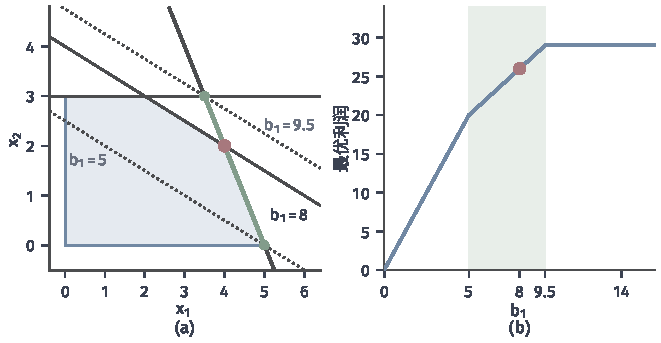
\includegraphics[width=112mm]{figures/05-optimization/01-linear-programming/matplotlib/simplex-rhs-range/figure.pdf}
 \caption{原料$b_1$的有效范围。(a)~实线和点线是$b_1=8$及范围两端$b_1=5,9.5$的原料线，绿色线段是最优顶点随$b_1$滑过的路径，红点是$b_1=8$的最优点。(b)~最优利润随$b_1$的变化（蓝线，对每个$b_1$精确求解），绿色底是基$(1,5,2)$的有效范围，其中斜率恒为影子价格$2$，范围之外斜率改变。}
 \label{fig:simplex-rhs-range}
\end{BookInlineFigure}

\paragraph{影子价格}
在有效范围内，$y_i$就是目标对$b_i$的变化率。按最大化利润的语言，它的相反数是多一单位资源带来的额外利润，称为\term{影子价格}（shadow price）。例中
\[
 -y_1^\star=2,\qquad -y_2^\star=1,\qquad -y_3^\star=0.
\]
一单位原料值$2$，一单位工时值$1$，设备还有富余，增加设备不值钱。如果市场上原料的单价低于$2$，就值得购买，但这个判断只在$b_1\leq9.5$之内有效。超过这个范围，图~\ref{fig:simplex-rhs-range}(b)的斜率变成了$0$，因为此时专用设备成了新的瓶颈。“影子价格”是局部的，它是某个固定基上的数，不是资源的绝对价值。

\paragraph{目标系数变化}
设基变量$x_k$的成本变化$\delta$，$k=B(\ell)$，$\bm{c}(\delta)=\bm{c}+\delta\bm{e}_k$。此时$\bm{x}$不变，对偶候选变化，由式~\eqref{eq:simplex-reduced-cost}计算得到
\begin{equation}
 s_j(\delta)=s_j-\delta\,\bar{a}_{\ell,j}\quad(j\in N),
 \qquad
 f(\delta)=p^\star+\delta\,x_k^\star.
 \label{eq:simplex-cost-parametric}
\end{equation}
其中$\bar{a}_{\ell,j}$是第$\ell$行的系数。基保持最优的条件是$s_j(\delta)\geq0$。若变化的是非基变量$x_j$的成本，只影响它自己的$s_j$，最优基在$s_j+\delta\geq0$时不变。

以产品一的利润为例，$x_1$位于基的第$1$个位置，第$1$行的系数由式~\eqref{eq:simplex-final-inverse}的第一行得到，$\bar{a}_{1,3}=-\frac13$，$\bar{a}_{1,4}=\frac23$。于是
\[
 s_3(\delta)=2+\frac13\delta,\qquad s_4(\delta)=1-\frac23\delta.
\]
非负条件给出$\delta\in[-6,3/2]$。由$c_1=-4+\delta$，换成产品一的利润$p_1=4-\delta$，范围是$p_1\in[2.5,10]$。

图~\ref{fig:simplex-cost-range}说明了这个区间。利润向量转动时，等值线绕最优点转动，最优点保持不动，直到等值线与某条活动约束重合。$p_1=2.5$时利润向量平行于$(1,2)$，$p_1=10$时平行于$(2,1)$，两个端点正好是两条活动约束的法向。

\begin{BookInlineFigure}
 \centering
 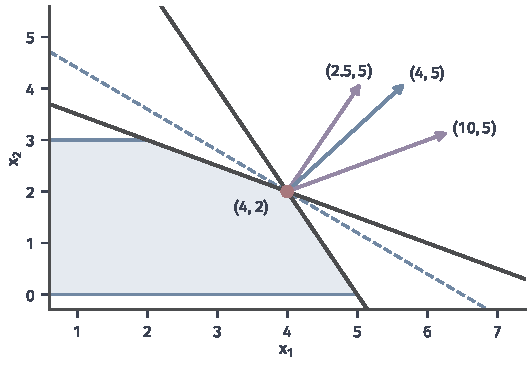
\includegraphics[width=90mm]{figures/05-optimization/01-linear-programming/matplotlib/simplex-cost-range/figure.pdf}
 \caption{产品一利润$p_1$的有效范围。深灰粗线是过$(4,2)$的两条活动约束，蓝色虚线是当前利润$p_1=4$的等值线。三支箭头只表示方向：蓝色是当前利润向量，紫色是范围端点$p_1=2.5$和$p_1=10$的利润向量，两者分别垂直于两条活动约束。}
 \label{fig:simplex-cost-range}
\end{BookInlineFigure}

表~\ref{tab:simplex-parameter-ranges}列出全部五个参数的结果。

\begin{BookInlineTable}
 \centering
 \begin{tabular}{cccl}
  \toprule
  参数 & 当前值 & 有效范围 & 变化率\\
  \midrule
  $b_1$ & $8$ & $[5,\ 9.5]$ & 利润$+2$\\
  $b_2$ & $10$ & $[7,\ 16]$ & 利润$+1$\\
  $b_3$ & $3$ & $[2,\ \infty)$ & 利润不变\\
  $p_1$ & $4$ & $[2.5,\ 10]$ & 利润$+x_1^\star=+4$\\
  $p_2$ & $5$ & $[2,\ 8]$ & 利润$+x_2^\star=+2$\\
  \bottomrule
 \end{tabular}
 \caption{单个参数变化时最优基$(1,5,2)$的有效范围，变化率指参数每增加一单位时最优利润的变化，只在范围内有效。}
 \label{tab:simplex-parameter-ranges}
\end{BookInlineTable}

几个参数同时变化时，结论要从向量形式读取。设右端变化$\Delta\bm{b}$，基$B$保持可行的条件是
\[
 \bar{\bm{x}}_B+\bm{A}_B^{-1}\Delta\bm{b}\geq\bm{0}.
\]
这是$\Delta\bm{b}$的一个多面体，不是逐个区间的乘积。把各个单独的范围同时用到极端，可能已经出界。

\paragraph{越出范围之后}
范围的端点不是答案的终点，只是这个基失效的位置。越过右端的范围，基失去原始可行性而保持对偶可行，这正是第~\ref{sec:simplex-dual}节的出发点。例如$b_1=11$时$x_5=-1$，对偶单纯形法一次换基就得到基$(1,3,2)$和解$(7/2,3)$，利润$29$，这与图~\ref{fig:simplex-rhs-range}(b)的平台一致。

越过目标系数的范围，基失去对偶可行性而保持原始可行，这时用原始单纯形法接着走。例如$p_1=12$时$s_3=-2/3$，$x_3$入基，$\bm{u}=(-1/3,-2/3,2/3)^\top$，比值检验给出$x_2$出基，点走到$(5,0)$，利润$60$。

把一个个基的有效范围拼起来，最优值就成为参数的分段线性函数，图~\ref{fig:simplex-rhs-range}(b)是一个例子，折点是换基发生的位置。在一般约束下，值函数和解映射如何随参数变化，由第~\ref{chap:parametric-sensitivity}章研究。

\section{最坏情形复杂度}
\label{sec:simplex-worst-case}

单纯形法有限终止，但有限不等于快。换基次数在最坏情况下能有多大，它和一次换基的代价是什么关系，实际表现又该怎样理解？

\paragraph{换基次数与每轮代价}
总运算量是两个因子的乘积：换基次数乘以每轮代价。第~\ref{sec:simplex-revised}节处理的是后者，稠密实现下每轮是$m$和$n$的低次多项式。本节讨论前者。基的个数最多是从$n$个下标中选$m$个的组合数，随规模指数增长，所以有限终止本身给不出多项式界。问题在于，算法会不会真的走那么多步。

\paragraph{Klee--Minty构造}
下面这族例子表明确实可能。第$n$个问题有$n$个变量和$n$个约束：
\begin{equation}
 \begin{aligned}
 \max\quad & z_n=\sum_{j=1}^n2^{n-j}x_j\\
 \text{s.t.}\quad & x_i+\sum_{j<i}2^{i-j+1}x_j\leq5^i,\quad i=1,\ldots,n,\\
 & \bm{x}\geq\bm{0}.
 \end{aligned}
 \label{eq:simplex-klee-minty}
\end{equation}
它属于Klee和Minty提出的压扁立方体构造\scite{math-klee1972simplex}。$n=2$时约束是$x_1\leq5$，$4x_1+x_2\leq25$，目标是$2x_1+x_2$。从原点出发，Dantzig规则选系数大的$x_1$，走到$(5,0)$；接着$x_2$入基，走到$(5,5)$；最后第一个松弛变量入基，走到$(0,25)$。四个顶点全被访问，如图~\ref{fig:simplex-klee-minty-plane}所示。

\begin{BookInlineFigure}
 \centering
 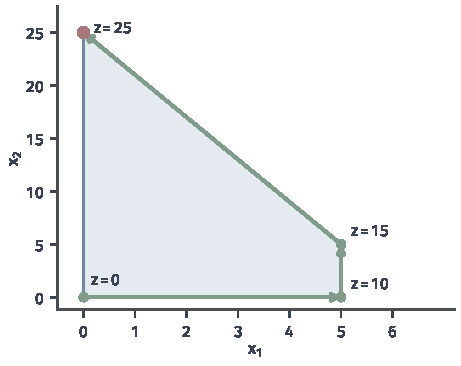
\includegraphics[width=78mm]{figures/05-optimization/01-linear-programming/matplotlib/simplex-klee-minty-plane/figure.pdf}
 \caption{$n=2$的Klee--Minty问题。可行域（浅蓝）有四个顶点，绿色路径依次访问全部四个，每个顶点旁标出目标值$z$，红点是最优解$(0,25)$。注意最优点其实与起点相邻，算法却绕了远路。}
 \label{fig:simplex-klee-minty-plane}
\end{BookInlineFigure}

$n=3$时情况相同，图~\ref{fig:simplex-klee-minty-cube}是可行域的示意。路径走完底面的四个顶点，上升一次，再把顶面的四个顶点反向走一遍。

\begin{BookInlineFigure}
 \centering
 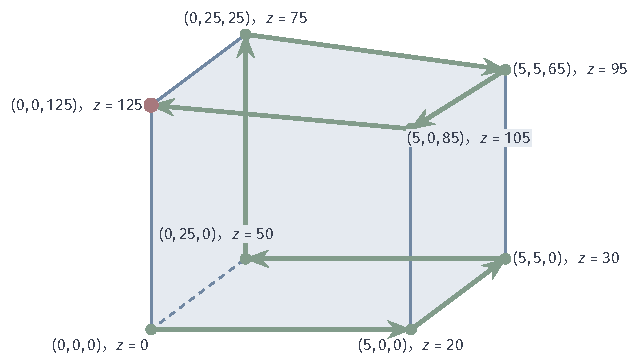
\includegraphics[width=108mm]{figures/05-optimization/01-linear-programming/tikz/simplex-klee-minty-cube/figure.pdf}
 \caption{$n=3$的Klee--Minty问题的示意，画成立方体，顶点坐标和目标值$z$是真实数据，比例不真实。绿色路径是Dantzig规则访问的顺序，共$7$次换基、走遍$8$个顶点，红点是最优解。}
 \label{fig:simplex-klee-minty-cube}
\end{BookInlineFigure}

这种“走完一面、再反着走一遍”的结构可以写成对$n$的归纳。为了写证明，先观察目标和约束之间的递推关系。记第$i$个松弛变量为$w_i$。由式~\eqref{eq:simplex-klee-minty}，第$n$个目标和第$n$个约束都可以用$z_{n-1}$表示：
\begin{equation}
 z_n=2z_{n-1}+x_n,\qquad w_n=5^n-x_n-4z_{n-1}.
 \label{eq:simplex-klee-minty-recursion}
\end{equation}
前$n-1$个约束恰好是第$n-1$个问题的约束，其中不含$x_n$和$w_n$。

下面用“字典”的语言：字典是把基变量和目标写成非基变量函数的表达式，也就是式~\eqref{eq:simplex-basic-form}和式~\eqref{eq:simplex-objective-form}的另一种叫法。最大化时，Dantzig规则选目标表达式中系数最大的正系数变量入基，这与最小化标准型中选最负的$s_j$是同一条规则。

\begin{theorem}[Klee--Minty问题的换基次数]
 \label{thm:simplex-klee-minty}
 对问题~\eqref{eq:simplex-klee-minty}，从全部松弛变量组成的基出发，Dantzig规则恰好经过$2^n-1$次换基到达最优解，最优值为$5^n$。
\end{theorem}

\begin{proof}
 对$n$归纳证明一个更强的命题。把从全松弛基出发、最大化$z_n$的运行称为上行，记为$U_n$；把从$U_n$的终点出发、最大化$-z_n$的运行称为下行，记为$D_n$。命题是：$U_n$和$D_n$各有$2^n-1$次换基；$U_n$过程中$z_n$从$0$增加到$5^n$，$D_n$过程中$z_n$从$5^n$减少到$0$并回到全松弛基；所有字典的目标系数都是整数。

 $n=1$时$z_1=x_1$，$w_1=5-x_1$。上行时$x_1$入基，一次换基后$z_1=5-w_1$。下行时目标是$-z_1=-5+w_1$，$w_1$入基，一次换基后$-z_1=-x_1$。命题成立。

 设命题对$n-1$成立，先看$U_n$。由式~\eqref{eq:simplex-klee-minty-recursion}，它分三段。

 第一段。设第$n-1$个问题的字典中$z_{n-1}$的系数为$d_k$，它们是整数。此时$z_n$的系数是$2d_k$，而$x_n$的系数是$1$。只要有$d_k>0$，就有$2d_k\geq2>1$，Dantzig规则的选择与$U_{n-1}$完全相同。第$n$行也不起限制作用，因为$x_n=0$且$z_{n-1}\leq5^{n-1}$，由式~\eqref{eq:simplex-klee-minty-recursion}得
 \[
  w_n\geq5^n-4\cdot5^{n-1}=5^{n-1}>0.
 \]
 所以算法照搬$U_{n-1}$，$2^{n-1}-1$次换基后$z_{n-1}=5^{n-1}$，所有$d_k\leq0$。

 第二段。此时只有$x_n$的系数为正，它入基。$x_n$只出现在第$n$行，所以$w_n$出基，$x_n=5^{n-1}$。这是一次换基。把$x_n=5^n-w_n-4z_{n-1}$代入$z_n$，目标变为
 \[
  z_n=5^n-w_n-2z_{n-1}.
 \]

 第三段。现在$w_n$的系数是$-1$，其余系数是$-2d_k$，后者正是$D_{n-1}$的目标$-z_{n-1}$放大$2$倍，$w_n$的系数为负，不会入基。第$n$行现在是$x_n=5^n-w_n-4z_{n-1}$，$w_n=0$时$x_n\geq5^{n-1}>0$，不起限制作用。所以算法照搬$D_{n-1}$，$2^{n-1}-1$次换基后$z_{n-1}=0$，所有系数非正，算法停止，此时$z_n=5^n$。

 三段合计$2(2^{n-1}-1)+1=2^n-1$次换基。

 再看$D_n$，它从$-z_n=-5^n+w_n+2z_{n-1}$开始，$z_{n-1}$的字典是全松弛基。第一段中$w_n$的系数是$1$，其余是$2d_k$，同样的比较说明算法照搬$U_{n-1}$，第$n$行$x_n\geq5^{n-1}>0$不起限制作用。第二段只有$w_n$的系数为正，它入基，$x_n$出基，代入后目标变为
 \[
  -z_n=-x_n-2z_{n-1}.
 \]
 第三段照搬$D_{n-1}$，第$n$行$w_n\geq5^{n-1}>0$不起限制作用，最后回到全松弛基，$z_n=0$。

 整数性由式~\eqref{eq:simplex-klee-minty-recursion}的递推保持，因为各段目标都是归纳假设中的整数系数乘$\pm2$再加上系数为$\pm1$的$x_n$或$w_n$。归纳完成。
\end{proof}

证明的要点在于系数的差距：前$n-1$个变量的系数翻倍，所以只要还有事可做，Dantzig规则就不会理会$x_n$；右端$5^i$的快速增长保证第$n$行不起限制作用。换一种规则结论就可能改变，图~\ref{fig:simplex-klee-minty-counts}(a)中Bland规则在这族例子上的步数少一些，但这只说明这族例子不是专门针对Bland规则构造的，其他构造同样能使Bland规则走指数多步。是否存在一条换基规则能保证多项式次换基，至今没有答案。

\begin{BookInlineFigure}
 \centering
 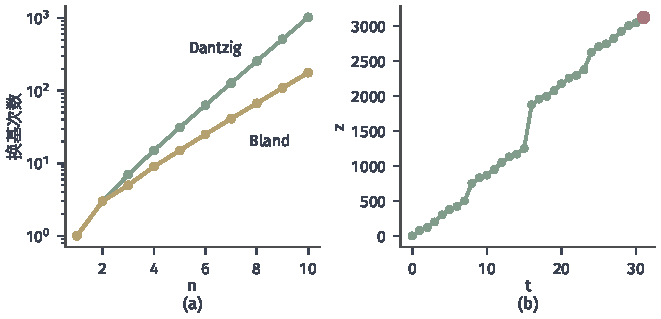
\includegraphics[width=112mm]{figures/05-optimization/01-linear-programming/matplotlib/simplex-klee-minty-counts/figure.pdf}
 \caption{Klee--Minty问题的实测结果，精确有理数运算。(a)~换基次数随$n$变化，纵轴取对数；绿线是Dantzig规则，恰为$2^n-1$；黄线是Bland规则。(b)~$n=5$时Dantzig规则各步的目标值，共$31$步，红点是最优值$3125$。}
 \label{fig:simplex-klee-minty-counts}
\end{BookInlineFigure}

\paragraph{最坏情形与实际表现}
定理~\ref{thm:simplex-klee-minty}是对一族特殊问题的结论，并不刻画算法在一般问题上的行为。长期的实践表明，单纯形法在大多数实际问题上的换基次数远小于组合数，常是约束数的不大的倍数。

图~\ref{fig:simplex-random-pivots}是一个小实验：$\bm{A},\bm{c}$的元素在$(0,1)$上独立均匀抽取，$\bm{b}=\bm{1}$，$m=n$，每种规模取$30$个随机种子。平均换基次数随规模温和增长，$m=320$时约$655$次，比Klee--Minty问题的指数增长慢得多。

\begin{BookInlineFigure}
 \centering
 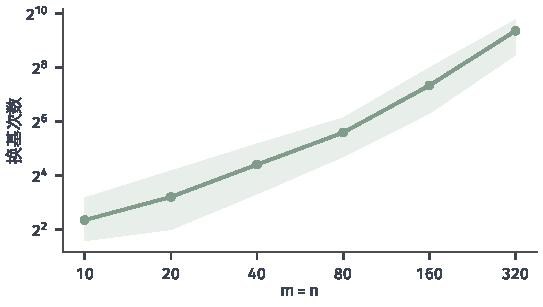
\includegraphics[width=92mm]{figures/05-optimization/01-linear-programming/matplotlib/simplex-random-pivots/figure.pdf}
 \caption{一种随机模型上Dantzig规则的换基次数，两轴都是对数刻度。绿线是$30$个随机种子的平均值，浅绿色带是最小值到最大值的范围。实验条件：$m=n$，$\bm{A},\bm{c}$的元素在$(0,1)$上独立均匀，$\bm{b}=\bm{1}$，起始基是全松弛基。}
 \label{fig:simplex-random-pivots}
\end{BookInlineFigure}

这个实验只说明这一随机模型上的情况，不能外推成对任意问题的保证。实际问题带有特定的结构，有时比随机模型容易，有时因退化严重而困难得多。理论上也有在特定随机扰动模型下给出多项式期望步数的结果，那些结论依赖扰动模型，并不告诉我们某一个具体实例要走多少步。

所以这里的两个判断要分开说：最坏情形下，Dantzig规则的换基次数可以随维数指数增长，这是定理；实际问题上换基次数通常不大，这是经验观察，没有无条件的平均复杂度保证。这个差别也是下一章研究多项式时间方法的原因之一。

\section{本章小结}
\label{sec:simplex-summary}

本章开头的问题是怎样在有限但极多的顶点之间找到最优的一个。单纯形法的回答是：用基来表示顶点，用约化成本判断哪条边值得走，用比值检验决定走多远，用对偶候选写出最优性证书。工厂的例子经过三次换基，从$(0,0)$走到$(4,2)$，并得到资源的对偶价格$(2,1,0)$。

算法的每个环节都有明确的条件。起步需要可行基，没有时用人工变量，两阶段法或符号化的大M法把它们排除；有限的$M$要超过对偶价格，这一点事先并不知道。退化基使步长为零，同一点对应多个基，循环可能发生，Bland规则或字典序规则在精确算术下保证有限终止。实现上修正单纯形法只维护基矩阵的因子，浮点运算要求小心选主元、定期重新分解，并在结束时重新核查。

算法的结果总是带着证据，表~\ref{tab:simplex-outcomes}汇总了三种停止结果。

\begin{BookInlineTable}
 \centering
 \begin{tabular}{lll}
  \toprule
  结果 & 检验 & 证据\\
  \midrule
  最优 & 可行基上$\bm{s}\geq\bm{0}$ & 原始解和对偶解，目标相等\\
  无界 & $s_q<0$且$\bm{u}\leq\bm{0}$ & 可行点和方向$\bm{d}$，$\bm{c}^\top\bm{d}<0$\\
  不可行 & 第一阶段$\phi^\star>0$，& $\bm{y}$，满足$\bm{A}^\top\bm{y}\leq\bm{0}$，$\bm{b}^\top\bm{y}>0$\\
  & 或对偶单纯形法无候选 & （后者取$\bm{y}=-\bm{\rho}$）\\
  \bottomrule
 \end{tabular}
 \caption{单纯形法的三种停止结果及其证据。}
 \label{tab:simplex-outcomes}
\end{BookInlineTable}

得到最优基以后，还能继续使用它。基的可行性和最优性分别管着右端和目标系数，固定基的参数分析读出每个参数的有效范围和影子价格；越出范围后，右端的变化交给对偶单纯形法，目标系数的变化交给原始单纯形法，只需少量换基。这种复用是单纯形法在整数规划等反复求解场合的重要优势。

有限终止不等于快。Klee--Minty构造说明Dantzig规则的换基次数最坏可以指数增长，实践中换基次数虽然通常不大，却没有无条件的理论保证。第~\ref{chap:lp-interior-point}章将研究另一条路线：不沿边界走，而从可行域内部逼近最优解。

